\documentclass[12pt]{article}
\usepackage[utf8]{inputenc}
\usepackage[T2A]{fontenc}
\usepackage[russian]{babel}
\usepackage{amsmath}
\usepackage{amssymb}
\usepackage{dsfont}
\usepackage[dvipsnames]{xcolor}
\usepackage{setspace}
\usepackage{multirow}
\usepackage[a4paper, outer=1.5cm, inner=1.5cm, top=1cm, bottom=1cm]{geometry}
\usepackage{graphicx}
\usepackage{skull}
\usepackage{wasysym}
\usepackage{float}
\graphicspath{{.images/}}
\usepackage{hyperref}
\hypersetup{colorlinks=true, linkcolor=blue, filecolor=magenta, urlcolor=cyan}
\usepackage[firstpage]{draftwatermark}
\SetWatermarkText{
    $\qquad\qquad\qquad\qquad\qquad$\parbox{7cm}{\begin{center}
    
\includegraphics[width = 0.08\textwidth]{lion-logo.png}\bigskip\\~\bigskip\\~\vspace{-24mm}\\~\end{center}}
}
\SetWatermarkAngle{0}
\SetWatermarkScale{1.5}
\usepackage{etoolbox}

\newtoggle{ifsolved}
\newtoggle{needhelp}
\newcounter{num}
\setcounter{num}{1}

\newcommand{\newnum}{\par\textbf{\textnumero\arabic{num}}\stepcounter{num}}
\newcommand{\sol}{\vspace{3mm}\par\textbf{Решение: }}
\newcommand{\ans}{\vspace{3mm}\par\textbf{Ответ: }}
\newcommand{\hint}{\vspace{3mm}\par\textbf{Подсказка: }}
\newcommand{\mode}[1]{
\ifstrequal{#1}{0}{\togglefalse{ifsolved}\togglefalse{needhelp}}{\ifstrequal{#1}{1}{\togglefalse{ifsolved}\toggletrue{needhelp}}{\ifstrequal{#1}{2}{\toggletrue{ifsolved}\togglefalse{needhelp}}{\toggletrue{ifsolved}\toggletrue{needhelp}}}}} %if 0 - if 1 - if 2 - else
%\newenvironment{problem}[8]{%#1, #2, #3
%\parbox{\linewidth}{\vspace{4mm}\ifstrequal{#4}{(лёгкая)}{\newnum\textbf{.}}{\newnum\textbf{*.} } \\ #5}
%\iftoggle{ifsolved}{\sol #6}{}
%\iftoggle{ifsolved}{\ans #7}{}
%\iftoggle{needhelp}{\hint #8}{}}

\newenvironment{problem}[8]{%#1, #2, #3
\parbox{\linewidth}{\vspace{5mm}\ifstrequal{#4}{(лёгкая)}{\newnum\textbf{.}}{\newnum\textbf{*.} } \\ #5}
\iftoggle{ifsolved}{\sol #6}{}

\iftoggle{ifsolved}{\parbox{\linewidth}{\ans #7}}{}
\iftoggle{needhelp}{\parbox{\linewidth}{\hint #8}}{}}

\newenvironment{mylist} %custom list
{ \begin{itemize}
    \setlength{\itemsep}{0pt}
    \setlength{\parskip}{0pt}
    \setlength{\parsep}{0pt}     }
{ \end{itemize}                  }

\newenvironment{homeass}[1]{\vspace*{-1.5cm}
\iftoggle{ifsolved}{
    \section*{\center{Решение домашнего задания к #1.}}
}{
    \section*{\center{\textcolor{Sepia}{Домашнее задание к #1}}}
} \vspace{7mm}\large}

\parindent=0pt
\pagestyle{empty}
%$\!$[\arabic{class}.\arabic{num}]
%\ifnumcomp{\value{counter}}{>}{1}{true}{false}
%\definecolor{Gray}{gray}{0.9}
%\definecolor{mypink}{RGB}{219, 48, 122}
%\newcolumntype{g}{>{\columncolor{Gray}}p{2.8cm}}

\begin{document}
\large
\mode{7}
%0 for problems without hints
%1 for problems + hints
%2 for problems + solutions + answers
%else: show all

{\centering\section*{СПИСОК ЗАДАЧ}}

{\centering\subsection*{\smallskip\\\textcolor{green}{\textbf{Полезные вещи, которые можно и нужно копипастить:}}}}

\subsection*{\textcolor{Emerald}{\textbf{Полезные шпаргалки по LaTeXу:}}}

\textbf{Пример вставки рисунка:}

\begin{minipage}{\linewidth}
    \begin{minipage}{0.54\linewidth}
    см. рисунок справа\\
    Текст к собственно пикче, примерно всегда это либо развёрнутое описание, либо большая часть решения задачи --- стремимся экономить пространство, если это можно сделать.
    \end{minipage}
    \hspace{0.05\linewidth}
    \begin{minipage}{0.4\linewidth}
    \begin{figure}[H] 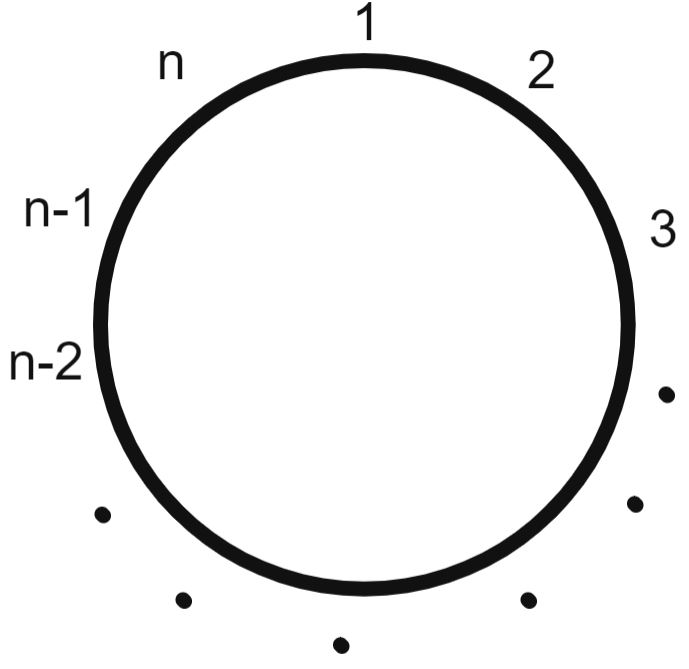
\includegraphics[width=\linewidth]{sol3} %тут поменять имя пикчи
    \end{figure}
    \end{minipage}
\end{minipage}

\textbf{Дефолтные математические знаки и символы:}\\
$\geqslant$,
$\leqslant$,
$a^{b}$,
$x_{i}$,
$\sqrt{a}$,
$\frac{a}{b}$,
$\displaystyle \frac{a}{b}$,
$\cdot$
$\;\Rightarrow\;$,
$\;\Leftrightarrow\;$,
$1{,}2$.
О промежутках:
$a\!b$,
$a\,b$,
$a\:b$,
$a\;b$,
$a\quad b$.

\textbf{Стандартные система и совокупность уравнений / неравенств:}\\
$\left\{
\begin{aligned}
f(x) &= 0 \\
g(x) &= 1
\end{aligned}\right.$

$\left[\begin{aligned}
&\left\{\begin{aligned}
f(x) &\geqslant a \\
g(x) &= b
\end{aligned}\right.\\
&\left\{\begin{aligned}
f(x) &< a \\
g(x) &= -b
\end{aligned}\right.
\end{aligned}\right.$

\subsection*{\textcolor{Emerald}{\textbf{Не математическое, но полезное:}}}
% комментарий в любом месте документа, который нигде не будет видно. Можно использовать для написания заметок-вопросов по задачам
\textbf{Пример таблицы:}

\begin{tabular}{|c|c|c|}
\hline
    $a$ & $b$ & текст
\\\hline
    $c$ & $d$ & мораль
\\\hline
\end{tabular}\\

\textbf{Отступы:} между\smallskip\\ строками\medskip\\ \textbf{Тире} --- это три дефиса.\\
\textbf{Списки:}
\begin{mylist}
\item [$\bullet$] это был пункт а
\item [2)] а это уже пункт номер 2 с изменённым заголовком
\end{mylist}

\subsection*{\textcolor{Emerald}{\textbf{Всё, неупомянутое выше (или если просто что-то не так):}}}
\begin{mylist}
\item [$\bullet$] Решение отдельных вопросов касательно ТеХа нужно искать в \href{https://www.mccme.ru/free-books/llang/newllang.pdf}{Львовском}.

\item [$\bullet$] Найти произвольный символ, который нужен, можно в \href{http://detexify.kirelabs.org/classify.html}{Detexify}.

\item [$\bullet$] Если возникли сомнения при решении, ответ практически ко всем задачам можно проверить с помощью \href{https://www.wolframalpha.com/}{WolframAlpha}.

\item [$\bullet$] Если в задаче нужно создать картинку, то лучше пока отложить эту задачу. Все графики планируется централизованно нарисовать (или перерисовать) в геогебре.

\item [\textcolor{brown}{\textbf{!!}}] Важно ставить \textcolor{red}{\textbf{$\spadesuit$}}
(или просто red) в тело задачи в случае серьёзных вопросов к решению и какой-то вопиющей лажи.

\item [\textcolor{brown}{\textbf{!!}}] Важно ставить \textcolor{olive}{\textbf{$\spadesuit$}}
(или просто olive) в тело задачи в случае не самого удачного текста и кривых отступов.
\end{mylist}

\subsection*{\textcolor{Violet}{\textbf{Комментарии:}}}% а также невидимые комментарии - так можно оставлять заметки-вопросы прямо в задаче, чтобы потом было понятно, в чём вопрос.
\begin{mylist}
\item [$\skull$] Переставлять задачи местами --- очень плохая идея.

\item [$\smiley$] При двойном клике по тексту pdf справа происходит автоматический переход к этому месту в латех-коде, а для обратного перехода можно нажать стрелку вправо (висит сверху между pdf и латех-кодом).

\item [$\smiley$] Если есть размышления, дописывать red/olive к задаче или не дописывать, то лучше всё-таки дописать.

\item [$\skull$] Самое плохое, что можно сделать --- написать в любое поле из трёх (НаписанноеРешение/ВерныйОтвет/Подсказка) только половину того, что надо, никак это не отметить, и потом пойти дальше.\\ Нужно в этот момент писать red/olive в случайном месте задачи, чтобы потом вычислить это с помощью Ctrl+F по всему документу (и это то, что потом будет делаться долго и тщательно)
\end{mylist}

\newpage
\setcounter{num}{164}

\hypertarget{6.5}{{\centering\section*{\bigskip\\\textcolor{Blue}{\hyperlink{start2}{\textcolor{Blue}{6.5}} Отношения и пропорциональность.}\vspace{-5mm}}}}

\begin{problem}{Отношения и пропорции.}{6.5.1}{6S}{(лёгкая)}
{Сумма трёх чисел равна $136{,}5$. Если первое число умножить на 8, второе~--- на 4, а третье~--- на 6, то полученные произведения окажутся равными.\\ Найти эти числа.}
{НаписанноеРешение}
{ВерныйОтвет}{Подсказка}
\end{problem}

\begin{problem}{Отношения и пропорции.}{6.5.1}{6S}{(лёгкая)}
{В трёх районах города 12000 жителей.\\ Сколько жителей в каждом районе, если известно, что $\frac{2}{3}$ числа жителей первого района равны $0{,}5$ жителей второго района и $\frac{2}{5}$ числа жителей третьего района?}
{НаписанноеРешение}
{ВерныйОтвет}{Подсказка}
\end{problem}

\begin{problem}{Отношения и пропорции.}{6.5.1}{6S}{(лёгкая)}
{В саду посадили 896 деревьев~--- яблонь, груш, и слив.\\ Яблони составляли $\frac{2}{7}$ всех деревьев. Сколько посадили груш и сколько~--- слив,\\ если на каждые 3 грушевых дерева приходилось 5 сливовых?}
{НаписанноеРешение}
{ВерныйОтвет}{Подсказка}
\end{problem}

\begin{problem}{Отношения и пропорции.}{6.5.1}{6S}{(лёгкая)}
{Разделить число 88 на 3 части пропорционально числам $\,\displaystyle\frac{1}{2}$, $\,\displaystyle\frac{3}{4}$, $\,\displaystyle1\frac{1}{2}$.}
{НаписанноеРешение}
{ВерныйОтвет}{Подсказка}
\end{problem}

\begin{problem}{Отношения и пропорции.}{6.5.1}{6K}{(лёгкая)}
{Пароход проходит расстояние между пунктами $A$ и $B$ и обратно за $3$ часа и $22{,}5$ минуты. Скорость парохода в стоячей воде $18$ км/ч, однако, пункты $A$ и $B$ стоят на реке, скорость течения которой равна $2$ км/ч.\\ Сколько километров от пункта $A$ до пункта $B$?}
{НаписанноеРешение}
{ВерныйОтвет}{Подсказка}
\end{problem}

\begin{problem}{Отношения и пропорции.}{6.5.1}{6S}{(лёгкая)}
{Три числа относятся, как $3 {:} 5 {:} 8$, третье число равно 112.\\ Найти два первых числа.}
{Если три числа относятся как $3 {:} 5 {:} 8$, это значит, что первое число составляет 3 каких-то неизвестных части, второе --- 5 таких частей, а третье --- 8 таких же частей. Поэтому одна часть в 8 раз меньше, чем 112 и равна $112 : 8 = 14$. Первое число содержит три таких части и потому равно $14 \cdot 3 = 42$, второе число содержит 5 $\;\Rightarrow\;$ оно равно 
$14\cdot 5 = 70$.}
{Первое число равно 42, второе число равно 70.}{Чему равна одна <<часть>>, которых в последнем числе целых восемь?}
\end{problem}

\begin{problem}{Отношения и пропорции.}{6.5.1}{6S}{(лёгкая)}
{Пять чисел относятся между собой как $1 : 2 : 3 : 4 : 5$. Найти эти числа, если:
\\a) Сумма первого и третьего чисел равна 40;
\\b) Разность между пятым числом и вторым равна 51.}
{НаписанноеРешение}
{ВерныйОтвет}{Подсказка}
\end{problem}

\begin{problem}{Отношения и пропорции.}{6.5.1}{6S}{(лёгкая)}
{Раздели число 144 на три части $x$, $y$, и $z$ так, чтобы $x {:} y = 3 {:} 4$, $\;y {:} z = 4 {:} 5$.}
{Если $x {:} y = 3 {:} 4$, а $\,y {:} z = 4 {:} 5$, то числа $x$, $y$, $z$ относятся как $3 {:} 4 {:} 5$. Значит, $x$, $y$ и $z$ вместе --- $3 + 4 + 5 = 12$ каких-то пока что неизвестных частей.\\ То есть мы получили, что 12 одинаковых частей --- 144. Следовательно, одна такая часть в 12 раз меньше и будет равна $144 : 12 = 12$.\\ В первом числе таких частей 3, и поэтому оно равно $12 \cdot 3 = 36$. Во втором числе частей четыре $\;\Rightarrow\; $ оно равно $12 \cdot 4 = 48$. Третье число равно $12 \cdot 5 = 60$.\\ Проверка: $x + y + z = 36 + 48 + 60 = 84 + 60 = 144$.}
{Эти три числа --- числа 36, 48, и 60.}{Пусть в первом числе три каких-то неизвестных части.\\ Сколько всего частей? Чему равна одна такая часть?}
\end{problem}

\begin{problem}{Отношения и пропорции.}{6.5.1}{6S}{(лёгкая)}
{Раздели число 310 на три части $x$, $y$, и $z$ так, чтобы $x {:} y = 3 {:} 2$, $\;y {:} z = 5 {:} 3$.}
{НаписанноеРешение}
{ВерныйОтвет}{Подсказка}
\end{problem}

\begin{problem}{Отношения и пропорции.}{6.5.1}{6S}{*}
{Раздели число 130 на три части так, чтобы удвоенная первая часть была равна утроенной второй части и четыре раза взятой третьей части.}
{НаписанноеРешение}
{ВерныйОтвет}{Подсказка}
\end{problem}

\begin{problem}{Отношения и пропорции.}{6.5.1}{6S}{(лёгкая)}
{Свежий гриб содержит 90\% воды, сушёный 12\%.\\ Сколько получится сушёных грибов из 10 кг свежих?}
{НаписанноеРешение}
{ВерныйОтвет}{Подсказка}
\end{problem}

\begin{problem}{Отношения и пропорции.}{6.5.1}{6S}{(лёгкая)}
{На складе хранилось 100 кг ягод, содержание воды в которых 99\%.\\ От долгого хранения содержание воды в ягодах сократилось до 98\%.\\ Сколько теперь весят ягоды?}
{НаписанноеРешение}
{ВерныйОтвет}{Подсказка}
\end{problem}

\begin{problem}{Отношения и пропорции.}{6.5.1}{6S}{(лёгкая)}
{Спортсменов сначала построили в колонны по $6$ человек, а потом перестроили на $4$ человека. Число рядов при этом увеличилось на $2$.\\ Сколько всего было спортсменов?}
{НаписанноеРешение}
{ВерныйОтвет}{Подсказка}
\end{problem}

\begin{problem}{Отношения и пропорции.}{6.5.1}{6S}{*}
{Какое число надо отнять одновременно от числителя и знаменателя дроби $\frac{29}{64}$, чтобы получить $\frac{2}{9}$?}
{Пусть $n$~--- число, которое отняли от числителя и знаменателя. Тогда: $$\frac{29 - n}{64 - n} = \frac{2}{9}$$
Это пропорция, решаем её: $\;9 \cdot (29 - n) = 2 \cdot (64 - n)$.\\ Раскроем скобки по распределительному закону: $\;261 - 9n = 128 - 2n$.\\ Переносим все неизвестные вправо, а числа влево: $261 - 128 = 9n - 2n \;\Rightarrow\\ 133 = 7n \; \Rightarrow n = 133 : 7 = 19$.\\ Проверка: $\quad\frac{29 - 19}{64 - 19} = \frac{10}{45} = \frac{2 \cdot 5}{9 \cdot 5} = \frac29$.}
{И от числителя, и от знаменателя надо отнять 19.}{Подсказка}
\end{problem}

\begin{problem}{Отношения и пропорции.}{6.5.1}{6S}{(лёгкая)}
{Найти дробь, равную $\displaystyle\frac{5}{7}$, сумма числителя и знаменателя которой равна $72$.}
{НаписанноеРешение}
{ВерныйОтвет}{Подсказка}
\end{problem}

\begin{problem}{Отношения и пропорции.}{6.5.1}{6S}{*}
{Какое число надо вычесть из числителя дроби $\frac{37}{63}$ и прибавить к её знаменателю, чтобы получилась дробь, равная $\frac{3}{17}$?}
{НаписанноеРешение}
{ВерныйОтвет}{Подсказка}
\end{problem}

\begin{problem}{Отношения и пропорции.}{6.5.1}{6K}{(лёгкая)}
{Решить пропорцию: $\;\displaystyle 6{,}5 : 16 = 4\frac{7}{8} : y$.}
{НаписанноеРешение}
{ВерныйОтвет}{Подсказка}
\end{problem}

\begin{problem}{Отношения и пропорции.}{6.5.1}{6K}{(лёгкая)}
{В саду на каждые $4$ яблони приходится $7$ дубов. Больше в саду ничего не растёт. Сколько всего яблонь, если в саду ровно $132$ дерева?}
{Поскольку на каждые 4 яблони приходится 7 дубов, это означает, что из 11 деревьев 4~--- яблони и 7~--- дубы. 132 дерева, которые находятся в саду~--- это 12 раз по 11 деревьев ($132 : 11 = 12$). То есть, пересчитав все деревья в саду, мы будем дюжину раз наблюдать по 4 яблони и 7 дубов, а значит всего яблонь в саду $4 \cdot 12 = 48$ штук, а дубов $7 \cdot 12 = 84$ штуки.}
{В саду 48 яблонь (и 84 дуба).}{Сколько деревьев из 11~--- яблони?}
\end{problem}

\begin{problem}{Отношения и пропорции.}{6.5.1}{6K}{(лёгкая)}
{Расстояние между двумя городами $200$ км. Автомобиль проехал $80\%$ этого расстояния за два с половиной часа. Найти (в км/ч) скорость автомобиля.}
{80\% от 200 км --- это $200 \cdot 0{,}8 = 20 \cdot 8 = 160$ км. Таким образом, данный автомобиль проезжает 160 км за $2{,}5$ часа. Значит, за 5 часов он проедет $160 \cdot 2 = 320$ километров. А за один час --- $320 : 5 = 64$ километра.}
{Скорость этого автомобиля составляет 64 км/ч.}{Какое расстояние проехал автомобиль?\\
А сколько бы он проехал за 5 часов?}
\end{problem}

\begin{problem}{Отношения и пропорции.}{6.5.1}{6K}{(лёгкая)}
{Расстояние между двумя складами $240$ км. Автомобиль проехал $62{,}5\%$ этого расстояния за $1$ час $40$ минут. Найти (в км/ч) скорость автомобиля.}
{НаписанноеРешение}
{ВерныйОтвет}{Подсказка}
\end{problem}

\begin{problem}{Отношения и пропорции.}{6.5.1}{6K}{(лёгкая)}
{Расстояние между городами $A$ и $B$ равно $105$ км. Автомобиль проехал $\frac57$ этого расстояния за полтора часа. Найти (в км/ч) скорость автомобиля.}
{Раз автомобиль проехал только $\frac57$ расстояния между городами, это значит, что он проехал $105 \cdot \frac57 = \frac{\textcolor{violet}{105} \cdot 5}{\textcolor{violet}{7}} = \frac{15 \cdot 5}{1} = 75$ километров. Всего автомобиль ехал полтора часа, значит это расстояние в полтора раза больше того, которое автомобиль проезжает за час, то есть за час он проедет $75 : 1{,}5 = 75 : \frac32 = 75 \cdot \frac23 = \frac{\textcolor{blue}{75} \cdot 2}{\textcolor{blue}{3}} = 50$ километров. Следовательно, скорость автомобиля~--- 50 км/ч.}
{Скорость автомобиля составляет 50 км/ч.}{Какое расстояние проехал автомобиль?}
\end{problem}

\begin{problem}{Отношения и пропорции.}{6.5.1}{6K}{*}
{Город А и город Б соединены прямой дорогой.\\
Известно, что жулик в настоящий момент быстро выезжает на машине из города А в город Б и с его скоростью он будет в Б через 3 часа 20 минут. Чтобы догнать его, хотели выслать машину, однако, понимая, что он едет слишком быстро, было решено выслать из города Б в город А, навстречу жулику, вертолет, который может пролететь все расстояние между А и Б за 2 часа 48 минут (считаем, что они покинули города одновременно). Через 1 час 15 минут между вертолетом и автомобилем с жуликом было ровно 100 км.\\ Какова скорость жулика? А какая скорость у вертолета?}
{Чтобы проехать всё расстояние между городами, жулику понадобится 3 часа 20 минут $= 3 \cdot 60 + 20 = 200$ минут. Вертолёт же может преодолеть расстояние между городами за $2 \cdot 60 + 48 = 168$ минут.\\ Поскольку прошло 75 минут, и жулик, и вертолёт пройдут лишь часть расстояния: жулик проедет $\frac{75}{200}$ всего расстояния, а вертолёт --- $\frac{75}{168}$. Выясним, какую часть расстояния между А и Б они проехали: $\frac{75}{200} + \frac{75}{168} = \frac{3}{8} + \frac{25}{56} = \frac{3\cdot7 + 25}{56} = \frac{46}{56} = \frac{23}{28}$.\smallskip\\ Значит, к этому моменту они ещё не встретились, и между ними ещё находится $1 - \frac{23}{28} = \frac{5}{28}$ пути. Как нам известно, это расстояние составляет ровно 100 км, а значит $\frac{1}{28}$ пути в 5 раз меньше и составляет 20 км, а расстояние между городами равно $20 \cdot 28 = 560$ км. Составим пропорцию и найдём скорости обоих участников:\smallskip\\
Жулик: 
$\quad\;\begin{aligned}
\text{200 минут}& \text{ --- 560 км}\\
\text{60 минут}& \text{ --- ? км}
\end{aligned} \;\Rightarrow\; 560 \cdot \frac{60}{200} = 560\cdot\frac{3}{10} = 56\cdot3 = 168$ км (за час).\smallskip\\
Вертолёт: 
$\;\:\begin{aligned}
\text{168 минут}& \text{ --- 560 км}\\
\text{60 минут}& \text{ --- ? км}
\end{aligned} \;\Rightarrow\; 560 \cdot \frac{60}{168} = 560\cdot\frac{15}{42} = 40\cdot5 = 200$ км (за час).}
{Скорость жулика --- 168 км/ч, скорость вертолёта --- 200 км/ч.}{Какая часть расстояния останется между ними через 75 минут?\\ Чему равно расстояние между городами А и Б? Составь и реши пропорцию, чтобы найти скорости обоих участников.}
\end{problem}

\begin{problem}{Отношения и пропорции.}{6.5.1}{6K}{*}
{Яблоко плавает на воде так, что в любой момент времени 1/5 часть яблока находится над водой, а 4/5~--- под водой.\\ Под водой яблоко начинает есть рыбка со скоростью 120 г/мин., одновременно над водой яблоко начинает есть птичка со скоростью 60 г/мин.\\ Какая часть яблока достанется рыбке, а какая~--- птичке?}
{НаписанноеРешение}
{ВерныйОтвет}{Подсказка}
\end{problem}

\begin{problem}{Отношения и пропорции.}{6.5.1}{6K}{(лёгкая)}
{Одно число больше другого числа на $\displaystyle 1\frac{1}{2}$, причём $\displaystyle\frac{1}{5}$ часть первого числа равна $\displaystyle\frac{1}{7}$ второго числа. Найти эти числа.}
{НаписанноеРешение}
{ВерныйОтвет}{Подсказка}
\end{problem}

\begin{problem}{Отношения и пропорции.}{6.5.1}{6K}{*}
{Из двух сплавов с $60$-процентным и $80$-процентным содержанием меди требуется получить $40$ кг сплава с $75$-процентным содержанием меди.\\ Какое количество каждого сплава нужно взять для этого?}
{НаписанноеРешение}
{ВерныйОтвет}{Подсказка}
\end{problem}

\begin{problem}{Отношения и пропорции.}{6.5.1}{6K}{(лёгкая)}
{Расстояние между двумя городами $907{,}5$ км.\\ Автомобиль проехал $60\%$ этого расстояния за четыре с половиной часа.\\ Найти (в км/ч) среднюю скорость автомобиля.}
{НаписанноеРешение}
{ВерныйОтвет}{Подсказка}
\end{problem}

\begin{problem}{Отношения и пропорции.}{6.5.1}{6K}{(лёгкая)}
{Расстояние между двумя населёнными пунктами $300$ км. Автомобиль проехал $91\%$ этого расстояния за $2$ часа $20$ минут. Какова скорость автомобиля?}
{НаписанноеРешение}
{ВерныйОтвет}{Подсказка}
\end{problem}

\begin{problem}{Отношения и пропорции.}{6.5.1}{6K red в рациональные числа, т.к. есть отрицательные}{*}
{Реши уравнение: $\displaystyle\;\frac{20x}{-2{,}8} + \frac{12}{2{,}1} = 0$.}
{При решении уравнений нужно отделить неизвестные от известных: поэтому можно <<перенести>> $\frac{12}{2{,}1}$ в правую часть уравнения (проще говоря, мы вычитаем $\frac{12}{2{,}1}$ из обеих частей уравнения~--- оно при этом остаётся верным).\\
Получаем, что $\displaystyle\;\frac{20x}{-2{,}8} = -\frac{12}{2{,}1}$. Домножим обе части уравнения на $-2{,}8$, для того, чтобы при $x$ не было дроби, а потом поделим обе части уравнения на 20. Итого: $$\displaystyle\; \frac{20x}{-2{,}8} = -\frac{12}{2{,}1} \;\Rightarrow\; 20x  = \left(\!-\frac{12}{2{,}1}\right) \cdot \left(-2{,}8\right) \;\Rightarrow\; x = \frac{12}{2{,}1} \cdot 2{,}8 : 20.$$
Вычислим, что же получилось справа: $\displaystyle \frac{12}{2{,}1} \cdot 2{,}8 : 20 = \frac{12 \cdot 2{,}8}{2{,}1 \cdot 20} = \frac{12\cdot4}{3\cdot20} = \frac45 = 0{,}8$.\\
Следовательно, $x = 0{,}8$ (или $x = \frac45$). Это и есть решение нашего уравнения.}
{Решением уравнения является $x = 0{,}8$.}{Для начала стоит вычесть из обеих частей уравнения $\frac{12}{2{,}1}$.}
\end{problem}

\begin{problem}{Отношения и пропорции.}{6.5.1}{6K}{(лёгкая)}
{Расстояние между двумя городами $150$ км.\\ Автомобиль выехал из первого города и проехал $42$ км за $22$ с половиной минуты.\\ Какое расстояние будет между ним и вторым городом через $52{,}5$ минуты?}
{Если автомобиль проезжает 42 километра за $22{,}5$ минуты, за $7{,}5$ минут он проедет 14 километров (за втрое меньшее время --- втрое меньшее расстояние). Отметим, что $52{,}5 = 7{,}5 \cdot 7$, и поэтому за 52 с половиной минуты --- в семь раз большее время --- автомобиль проедет в семь раз больше, то есть $14 \cdot 7 = 98$ километров. Получается, автомобиль проехал $42 + 98 = 140$ километров. Расстояние между первым и вторым городами составляет 150 км, а значит в этот момент расстояние между автомобилем и вторым городом будет равно $150 - 140 = 10$ км.}
{Между автомобилем и вторым городом будет расстояние 10 км.}{Сколько проезжает автомобиль за $7{,}5$ минут?}
\end{problem}

\begin{problem}{Отношения и пропорции.}{6.5.1}{6K}{*}
{Периметр прямоугольника равен $84$ см.\\ Найти его площадь, если стороны относятся как $5 {:} 7$.}
{Полупериметр этого прямоугольника (половина периметра) равен 42 сантиметрам. Это означает, что сумма длины и ширины этого прямоугольника равна $42$ см. Осталось разделить 42 в отношении $5 {:} 7$. Если ширина составляет 5 неизвестных частей, а длина --- 7 неизвестных частей, то вместе они составляют 12 таких частей. То есть $12$ частей --- 42 см, а значит, одна часть --- в 12 раз меньше, и равна $42 : 12 = 7 : 2 = 3{,}5$ см. Получается, что ширина составляет 5 таких частей и имеет длину $5\cdot3{,}5 = 17{,}5$ см, а длина имеет длину $7 \cdot 3{,}5 = 24{,}5$ см.\\
Площадь любого прямоугольника, в том числе и этого, равна произведению длины на ширину: $S = 17{,}5 \cdot 24{,}5 = \frac{35}{2}\cdot\frac{49}{2} = \frac{1715}{4} = 428{,}75$ см$^2$.}
{Площадь этого прямоугольника составляет $428{,}75$ см$^2$.}{Чему равна сумма длины и ширины?\\ Подели это число в отношении $5{:}7$, найди стороны, и вычисли площадь.}
\end{problem}

\begin{problem}{Отношения и пропорции.}{6.5.1}{6K}{(лёгкая)}
{Разделить $75$ на два числа так, чтобы большее число было в $3$ раза больше, чем разность между этими двумя числами.}
{НаписанноеРешение}
{ВерныйОтвет}{Подсказка}
\end{problem}

\begin{problem}{Отношения и пропорции.}{6.5.1}{6S}{(лёгкая)}
{Имеются брёвна двух видов: длиной 6 метров и длиной 7 метров. Их нужно распилить на метровые чурбаки, и один распил занимает 1 минуту.\\ Какие брёвна пилить выгоднее по времени?}
{НаписанноеРешение}
{ВерныйОтвет}{Подсказка}
\end{problem}

\begin{problem}{Отношения и пропорции.}{6.5.1}{6S}{(лёгкая)}
{Две официантки заработали вместе 20880р. Одна работала 7 дней по 6ч в день, другая 5 дней по 9ч. Сколько заработала каждая официантка, если всю оплату они разделили между собой по затратам рабочего времени?}
{<<Официантки разделили оплату между собой по затратам рабочего времени>>. А каковы эти затраты? Первая официантка отработала $7 \cdot 6 = 42$ часа, а вторая $5 \cdot 9 = 45$ часов. То есть всего они отработали $42 + 45 = 87$ часов, из которых 42 часа~--- часы первой официантки, а 45~--- часы второй официантки. Значит, общую сумму в 20880 рублей заплатили за 87 часов работы.\\ Сколько тогда стоил один час? В 87 раз меньше: $20880 : 87 = 240$ рублей.\\ Тогда первая официантка должна получить $240 \cdot 42 = 10080$ рублей, а вторая~--- $240 \cdot 45 = 10800$ рублей.}
{Первая заработала 10080 рублей, а вторая~--- 10800 рублей.}{За сколько всего рабочих часов заработали?\\ Сколько в таком случае платят за один час работы?}
\end{problem}

\begin{problem}{Отношения и пропорции.}{6.5.1}{6K}{(не лёгкая)}
{Пекарь продавал булочки и пирожки, и вот вечером, когда он уже собирался закрывать магазин, к нему зашёл покупатель и сказал, что он покупает все оставшиеся сладости. Пекарь был очень удивлён и спросил, кому покупаются все эти сладости, на что получил ответ:
\\<<Это на день рождения в школу для моих сыновей-тройняшек, они учатся в классах $2$А, $2$Б и $2$В. Я хочу разделить сладости пропорционально числу детей в каждом классе, чтобы каждому досталось поровну, и никто не обиделся~--- в классе $2$А учится $32$ школьника, в классе $2$Б~--- $25$, в классе $2$В~--- $28$>>. \\Таинственный покупатель ушёл, забрав все $10{,}2$ килограмм булочек и пирожков.\\ Сколько килограммов сладкого достанется каждому классу?}
{Сколько всего школьников получат сладости? В трёх классах всего учится $32 + 25 + 28 = 32 + 28 + 25 = 60 + 25 = 85$ человек. Сладости разделяются поровну, а значит на одного школьника придётся $10{,}2 : 85 = 102 : 850 = \frac{102}{850} = \frac{51}{425} = \frac{3}{25} = 0{,}12$ кг $= 120$ г. Тогда класс 2А получит $32 \cdot 0{,}12 = 3{,}84$ кг сладкого, класс 2Б --- $25 \cdot 0{,}12 = 3$ килограмма, а класс 2В --- $28 \cdot 0{,}12 = 3{,}36$ кг.}
{3 килограмма 840 грамм сладкого отправится в класс 2А, 3 килограмма сладостей --- в класс 2Б, 3 килограмма 360 грамм --- в класс 2В.}{Сколько всего школьников?\\ Если делить сладкое поровну между ними, то сколько достанется каждому?}
\end{problem}

\begin{problem}{Отношения и пропорции.}{6.5.1}{6S}{(лёгкая)}
{Из двух поездов один затрачивает на прохождение пути между двумя городами 2 ч 48 мин, другой~--- 4 ч 40 мин. Скорость первого поезда больше скорости второго на 26 км/ч. Определи расстояние между городами.}
{НаписанноеРешение}
{ВерныйОтвет}{Подсказка}
\end{problem}

\begin{problem}{Отношения и пропорции.}{6.5.1}{6K}{*}
{Некто едет по своему дому на лифте и спускается с 9 этажа на первый за 24 секунды. Сколько понадобится секунд лифту, чтобы спуститься с 3 этажа на первый?\\ (При решении считать, что лифт стартует мгновенно, и его скорость во время движения постоянна)}
{НаписанноеРешение}
{ВерныйОтвет}{Подсказка}
\end{problem}

\begin{problem}{Отношения и пропорции.}{6.5.1}{6S}{*}
{Машинист пассажирского поезда проехал туннель за 7 мин 30 с, а его коллега, водивший товарные поезда, проехал тот же туннель за 9 мин 30 с. Скорость пассажирского поезда на 4 м/с больше, чем товарного. Какова длина туннеля?}
{НаписанноеРешение}
{ВерныйОтвет}{Подсказка}
\end{problem}

\begin{problem}{Прямая и обратная пропорциональность.}{6.5.2}{6K}{(лёгкая)}
{Петя едет на велосипеде со скоростью $12$ км/ч.\\ Сколько километров он проедет за $20$ минут?}
{НаписанноеРешение}
{ВерныйОтвет}{Подсказка}
\end{problem}

\begin{problem}{Прямая и обратная пропорциональность.}{6.5.2}{6K}{(лёгкая)}
{Микола по выходным ездит на ярмарку. Если он едет на телеге, то путь туда-обратно занимает у него $5$ часов. Сегодня на выезде с ярмарки у него подломилась ось, и он возвращался домой пешком. Из-за этого на путь туда-обратно он потратил $10$ часов. Сколько бы занял у Миколы путь туда и обратно, если бы он всю дорогу шёл пешком?}
{НаписанноеРешение}
{ВерныйОтвет}{Подсказка}
\end{problem}

\begin{problem}{Прямая и обратная пропорциональность.}{6.5.2}{6K}{(лёгкая)}
{$10$ преподавателей проверяли $210$ задач $4$ часа. За сколько часов восемь из этих преподавателей смогли бы проверить $252$ задачи?}
{Если бы преподавателей было в 10 раз меньше, они бы за то же время проверили в 10 раз меньше задач. Следовательно, 1 преподаватель проверяет 21 задачу 4 часа. Тогда 8 преподавателей проверяют за 4 часа в 8 раз больше, а именно $8 \cdot 21 = 168$ задач. Однако, преподавателям надо проверить не 168, а 252 задачи, что больше в $\frac{252}{168} = \frac{126}{84} = \frac{63}{42} = \frac{9}{6} = \frac32$ раза.\\ То есть, преподавателям нужно выполнить в полтора раза большую работу~--- а значит и времени им потребуется в полтора раза больше, то есть $4 \cdot \frac32 = 6$ часов.}
{8 преподавателей проверят 252 задачи за 6 часов.}{Во сколько раз уменьшилось число преподавателей и во сколько раз увеличилось количество задач?}
\end{problem}

\begin{problem}{Прямая и обратная пропорциональность.}{6.5.2}{6K}{(лёгкая)}
{Три синих попугая капитана Флинта съедают три килограмма корма за три дня, пять зелёных попугаев~--- пять килограмм корма за пять дней, а семь оранжевых~--- семь килограмм корма за неделю.\\ Какие попугаи самые прожорливые и во сколько раз они прожорливее остальных?

}
{Один синий попугай съедает втрое меньше корма, чем три синих попугая. Поэтому один синий попугай съест килограмм корма за 3 дня.\\
Аналогично, один зелёный попугай съедает килограмм корма за 5 дней.\\
А один оранжевый попугай съедает килограмм корма за 7 дней.\smallskip\\
Поэтому становится понятно, что самые прожорливые~--- синие попугаи, поскольку синий попугай съедает килограмм корма быстрее прочих попугаев. Он съедает его в $\frac53$ раза быстрее, чем зелёный попугай, и в $\frac73$ раза быстрее, чем оранжевый.}
{Самые прожорливые попугаи у капитана Флинта~--- синие.\\ Они прожорливее зелёных в $\frac53$ раза и оранжевых в $\frac73$ раза.}{Сравни, за какое время съедает килограмм корма каждый попугай. Кто ест быстрее всех~--- тот и самый прожорливый.}
\end{problem}

\begin{problem}{Прямая и обратная пропорциональность.}{6.5.2}{6K}{(лёгкая)}
{6 голодных котов в амбаре, полном мышей, ловят $10$ мышей за $60$ минут.\\ Сколько мышей поймают $16$ голодных котов за $90$ минут?}
{НаписанноеРешение}
{ВерныйОтвет}{Подсказка}
\end{problem}

\begin{problem}{Прямая и обратная пропорциональность.}{6.5.2}{6K}{*}
{Куб размером $3 \times 3 \times 3$ разрезали на $27$ кубиков размером $1 \times 1 \times 1$ сантиметр. Известно, что для покраски всей поверхности куба $3 \times 3 \times 3$ нужно $28$ грамм краски. Сколько грамм краски нужно для того, чтобы покрасить все $27$ маленьких кубиков со всех шести сторон?}
{Для того чтобы понять, сколько краски уйдёт на обкрашивание всех кубиков со всех сторон, надо понять, на покраску чего уходит 28 грамм краски.\\
Куб, состоящий из 27 кубиков, с каждой своей стороны имеет $3\cdot3 = 9$ граней маленьких кубиков (достаточно представить кубик Рубика). И все эти грани будут раскрашены. Значит, их всего будет $6\cdot 9 = 54$ штуки (у большого куба 6 больших граней, и на каждой из них по 9 граней маленьких кубиков мы раскрашиваем).\\
Если же нам надо будет покрасить каждый из 27 маленьких кубиков со всех шести сторон, то всего надо будет покрасить $27 \cdot 6 = 162$ маленьких грани.\\ Это втрое больше, чем $54$ грани, так как $162 : 54 = 3$.\\ Следовательно, и краски понадобится втрое больше, а именно $28 \cdot 3 = 84$ грамма.}
{На покраску всех кубиков со всех сторон уйдёт 84 грамма краски.}{Сколько граней маленьких кубиков красится в каждом случае?}
\end{problem}

\begin{problem}{Прямая и обратная пропорциональность.}{6.5.2}{6K}{(лёгкая)}
{Цена билета на аттракцион составляет $15$ евро. Когда цену понизили, количество людей, посетивших аттракцион, возросло на $50\%$, а сбор денег увеличился на $25\%$. На сколько евро понизили стоимость билета?}
{НаписанноеРешение}
{ВерныйОтвет}{Подсказка}
\end{problem}

\begin{problem}{Прямая и обратная пропорциональность.}{6.5.2}{6K}{(лёгкая)}
{Кролики, живущие в вольере, съедают $100$ мини-морковок за два дня.\\ За сколько дней кончится мешок морковок ($850$ штук)?}
{НаписанноеРешение}
{ВерныйОтвет}{Подсказка}
\end{problem}

\begin{problem}{Прямая и обратная пропорциональность.}{6.5.2}{6K}{(лёгкая)}
{Турист вышел из дома в $08{:}47$. Он прошёл $8$ км за $120$ минут, и вдруг обнаружил, что забыл паспорт. Он побежал обратно домой в $5$ раз быстрее, чем шёл в начале. Во сколько он прибежит домой, если не выдохнется?}
{В данном случае видно, что в обратную сторону туристу нужно пройти то же расстояние, что он уже прошёл. Поэтому, если он побежит в 5 раз быстрее, чем шёл до этого, он преодолеет это расстояние за в 5 раз меньшее время, то есть за $120 : 5 = 24$ минуты. Поэтому на весь путь туда-обратно у туриста уйдёт 144 минуты, или 2 часа 24 минуты. $08{:}47 + 02{:}24 = 11{:}11$.\\
Таким образом, в этот момент на часах будет $11{:}11$.}
{Этот турист прибежит домой в $11{:}11$.}{Сколько минут турист будет бежать обратно?}
\end{problem}

\begin{problem}{Прямая и обратная пропорциональность.}{6.5.2}{6K}{(лёгкая)}
{В команде есть эрудиты и зазнайки, всего $15$ человек. Слова отгадывают только эрудиты. После того, как из команды ушло два эрудита и трое зазнаек, количество отгадываемых слов уменьшилось вдвое. Сколько зазнаек осталось в команде?}
{Поскольку слова отгадывают только эрудиты, и после ухода двух эрудитов команда стала отгадывать вдвое меньше слов, это означает, что количество эрудитов уменьшилось вдвое. Значит, два ушедших из команды эрудита --- половина от тех эрудитов, что были в команде изначально, и в команде было 4 эрудита.\smallskip\\ Поэтому изначально в команде было $15 - 4 = 11$ зазнаек, а после того, как трое ушло, зазнаек осталось 8.}
{В команде осталось 8 зазнаек.}{Если количество угадываемых слов уменьшилось вдвое, то во сколько раз уменьшилось число эрудитов? Сколько их было? А сколько было зазнаек?}
\end{problem}

\begin{problem}{Прямая и обратная пропорциональность.}{6.5.2}{6K}{(лёгкая)}
{$3$ землекопа выкапывают $3$ ямы за $2$ часа.\\ Сколько ям выкопают $6$ землекопов за $5$ часов?}
{НаписанноеРешение}
{ВерныйОтвет}{Подсказка}
\end{problem}

\begin{problem}{Прямая и обратная пропорциональность.}{6.5.2}{6K}{(лёгкая)}
{С помощью 6 одинаковых труб бассейн заполняется водой за $15$ часов.\\ На сколько часов раньше заполнится этот же бассейн, если труб станет на три больше?}
{Когда труб станет на 3 больше, их будет 9. Если сейчас труб станет вдвое меньше, то на заполнение бассейна у них уйдёт вдвое больше времени: то есть 3 трубы заполняют бассейн за 30 часов. Если же труб станет 9, то есть втрое больше, чем 3, то время, необходимое для заполнения бассейна, уменьшится втрое. Значит, 9 труб заполнят бассейн за 10 часов, что на 5 часов быстрее, чем 15.}
{Когда труб станет 9, наполнение бассейна будет занимать на 5 часов меньше времени.}{Сколько времени бы ушло, если бы труб было вдвое меньше?}
\end{problem}

\begin{problem}{Прямая и обратная пропорциональность.}{6.5.2}{6S}{(лёгкая)}
{15 плотников построили дом за 28 дней. За сколько дней 35 плотников построят 8 таких домов, если будут работать с такой же производительностью?}
{Если бы плотников было бы не 15, а 5, то из-за того, что их было бы втрое меньше, у них бы ушло втрое больше времени, то есть $28 \cdot 3 = 84$ дня.\\ Таким образом, 5 плотников строят 1 дом за 84 дня.\\ Если бы плотников было бы в 7 раз больше, у них бы ушло в 7 раз меньше времени, поэтому 35 плотников могут построить 1 дом за $84 : 7 = 12$ дней.\\ На 8 домов понадобится в 8 раз больше времени, а именно $12 \cdot 8 = 96$ дней.}
{35 плотников построят 8 домов за 96 дней.}{За какое время 5 плотников построят один дом?}
\end{problem}

\begin{problem}{Прямая и обратная пропорциональность.}{6.5.2}{6K}{(лёгкая)}
{Четверо рабочих проводили работы по замене асфальтного покрытия у дома №$19$ и закончили их за $27$ часов. На сколько часов дольше заменяли бы асфальтное покрытие, если бы рабочих было на одного меньше?}
{Если бы рабочих было бы на одного меньше, их было бы трое. То есть число рабочих составляло бы $\frac34$ от того количества рабочих, которое справилось закончить работы за 27 часов. В этом случае необходимое время было бы больше в $\frac43$ раза (поскольку с уменьшением числа рабочих во сколько-то раз, требуемое время во столько же раз увеличится). Таким образом, трём рабочим бы понадобилось $27 \cdot \frac43 = 36$ часов, или на 9 часов больше, чем 27 часов.}
{Если бы рабочих было на одного меньше, то асфальтное покрытие у дома №19 заменяли бы на 9 часов дольше.}{Во сколько раз уменьшилось число рабочих?}
\end{problem}
\begin{problem}{Прямая и обратная пропорциональность.}{6.5.2}{6K}{(лёгкая)}
{$100$ котов ловят $100$ мышей за $100$ дней. За сколько дней $2$ кота поймают $3$ мыши?

}
{НаписанноеРешение}
{ВерныйОтвет}{Подсказка}
\end{problem}

\begin{problem}{Прямая и обратная пропорциональность.}{6.5.2}{6K}{*}
{Оркестр из 30 музыкантов исполняет 6-ю симфонию Бетховена за 40 минут.\\ За какое время оркестр из 60 музыкантов исполнит 12-ю симфонию Бетховена?}
{Первый, самый главный вопрос, который надо себе задавать в любой задаче~--- что происходит? Оркестр увеличился, музыкантов стало вдвое больше.\\
Начнут ли музыканты после этого играть вдвое быстрее? Разумеется, нет!\\ Музыка~--- это искусство, <<поспешишь~--- людей насмешишь>>. То есть величина оркестра влияет на насыщенность звука, но никак не на скорость исполнения.\\ Мы знаем, что \href{https://ru.wikipedia.org/wiki/\%D0\%A1\%D0\%B8\%D0\%BC\%D1\%84\%D0\%BE\%D0\%BD\%D0\%B8\%D1\%8F\_\%E2\%84\%96\_6\_(\%D0\%91\%D0\%B5\%D1\%82\%D1\%85\%D0\%BE\%D0\%B2\%D0\%B5\%D0\%BD)}{6-ю симфонию} исполняют 40 минут. Знаем ли мы, сколько времени исполняют 12-ю симфонию? Нет! Значит, на вопрос задачи без дополнительной информации мы ответить не сможем.}
{Нам неизвестно, сколько длится 12-я симфония Бетховена.\\ Более того, если заглянуть в энциклопедию, то можно узнать, что Бетховен написал всего 9 симфоний, так что оркестр играть вообще не будет.}{Что произойдёт, если музыкантов станет вдвое больше?}
\end{problem}

\begin{problem}{Прямая и обратная пропорциональность.}{6.5.2}{6K}{(лёгкая)}
{В прошлом году $11$ преподавателей составляли задачи к олимпиаде $18$ дней. В этом году они опять собрались составлять задачи, однако двое преподавателей не смогли поучаствовать. За сколько дней они составят задачи в этом году?}
{Поскольку двое преподавателей не смогли поучаствовать, в этом году составлением задач будет заниматься $11 - 2 = 9$ преподавателей. Если бы преподавателей было бы в 11 раз меньше, то понятное дело, у одного преподавателя ушло бы в 11 раз больше времени на то, чтобы составить все задачи (то есть $18 \cdot 11$ дней). Но в этом году преподавателей будет не 1, а 9, то есть они справятся в 9 раз быстрее, чем 1 преподаватель, а именно за $18 \cdot 11 : 9 = 2 \cdot 11 = 22$ дня.}
{В этом году 9 преподавателей составят задачи за 22 дня.}{Если преподавателей станет меньше, то им потребуется больше или меньше времени? Сколько дней нужно одному преподавателю, чтобы составить эти же задачи?}
\end{problem}

\begin{problem}{Прямая и обратная пропорциональность.}{6.5.2}{6K}{*}
{В стране гигантов все вещи в $4$ раза больше, чем в обычном мире (деревья в $4$ раза выше, реки в $4$ раза шире). Путешественники нашли большой пустой спичечный коробок. Сколько обычных спичечных коробков в него поместится?}
{Во-первых, большой спичечный коробок в 4 раза длиннее обычного. Во-вторых, он в 4 раза шире. И наконец, в-третьих, он в 4 раза выше. Значит, в него одновременно влезает 4 спичечных коробка по ширине, длине, и высоте. Тогда несложно догадаться, что всего коробков в основании большого коробка может поместиться $4\cdot4 = 16$ штук. А во всём большом коробке поместится в четыре раза больше (высота больше в 4 раза, таких слоёв будет 4) $\;\Rightarrow\; 4\cdot4\cdot4 = 16\cdot4 = 64$ штуки.}
{В него поместится 64 обычных спичечных коробка.}{По скольким направлениям, кроме длины, этот большой коробок в 4 раза больше, чем обычный?}
\end{problem}

\begin{problem}{Прямая и обратная пропорциональность.}{6.5.2}{6K}{(не лёгкая)}
{Куб со стороной $1$ м распилили на кубики со стороной $1$ см и положили в ряд.\\ Какой длины он получился?}
{Для того, чтобы понять, какой длины получится ряд, нужно понять, сколько всего в нём кубиков. В длину, ширину, и высоту получится по 100 кубиков (так как в одном метре 100 сантиметров). Поэтому в одном слое (грани) $100 \cdot 100 = 10000$ кубиков, а во всём кубе $100 \cdot 100 \cdot 100 = 10000 \cdot 100 = 1000000$ кубиков.\\ Так как один кубик имеет длину 1 сантиметр, длина этого ряда получится равной $1000000$ сантиметров. $1000000$ см $= 10000$ м $= 10$ км.}
{Данный ряд содержит миллион кубиков и будет иметь длину 10 км.}{Сколько всего кубиков в этом ряду?}
\end{problem}

\begin{problem}{Прямая и обратная пропорциональность.}{6.5.2}{6S}{(лёгкая)}
{Две бригады, работая вместе, могут выполнить некоторую работу за 6 дней.\\ Если же обе бригады будут работать вместе только $\frac{1}{2}$ этого срока, после чего одна из бригад прекратит работу, то второй бригаде для окончания работы понадобится ещё 5 дней.\\ За сколько дней эту работу может выполнить каждая бригада по отдельности?}
{НаписанноеРешение}
{ВерныйОтвет}{Подсказка}
\end{problem}

\begin{problem}{Прямая и обратная пропорциональность.}{6.5.2}{6K}{*}
{В бассейн проведена труба. Она засорилась, и в итоге приток воды уменьшился на 60\%. На сколько процентов из-за этого увеличится время, необходимое для заполнения бассейна? (других труб не было, нет, и не будет)}
{Если приток воды уменьшился на 60\%, это означает, что теперь воды притекает лишь $40\%$ от прежнего количества, или $\frac{40}{100} = \frac25$ от прежнего количества. Значит, количество воды уменьшилось в $\frac52 = 2{,}5$ раза. Тогда время на заполнение того же бассейна увеличится в $2{,}5$ раза и будет составлять $2{,}5 T$. Следовательно, по сравнению с начальным $T$, время выросло на $1{,}5 T$, или на 150\%.}
{Время увеличится на 150\%.}{Во сколько раз уменьшился приток воды?\\ Во сколько раз увеличилось время?}
\end{problem}

\begin{problem}{Прямая и обратная пропорциональность.}{6.5.2}{7A}{*}
{4 куртки стоят на 150\% дороже 10 рубашек.\\ На сколько процентов рубашка дешевле куртки?}
{НаписанноеРешение}
{ВерныйОтвет}{Подсказка}
\end{problem}

\begin{problem}{Прямая и обратная пропорциональность.}{6.5.2}{6K letovo}{*}
{Купец случайно перемешал конфеты первого сорта (по $300$ руб. за фунт) и конфеты второго сорта (по $200$ руб. за фунт).\\ По какой цене надо продавать эту смесь, чтобы выручить ту же сумму, если\\ известно, что первоначально общая стоимость всех конфет первого сорта была равна общей стоимости всех конфет второго сорта?}
{НаписанноеРешение}
{ВерныйОтвет}{Подсказка}
\end{problem}

\begin{problem}{Прямая и обратная пропорциональность.}{6.5.2}{9I}{*}
{\vspace{-12mm}\\\begin{minipage}{\linewidth}
    \begin{minipage}{0.62\linewidth}
    \vspace{12mm}
    
    Из чугуна изготовили тор (бублик), аналогичный изображённому на рисунке справа. \smallskip\\На сколько процентов больше будет вес точно такого же тора, все линейные размеры которого (длина, ширина и высота) будут увеличены на 10\%?

    \end{minipage}
    \hspace{0.04\linewidth}
    \begin{minipage}{0.33\linewidth}
        \begin{figure}[H]
        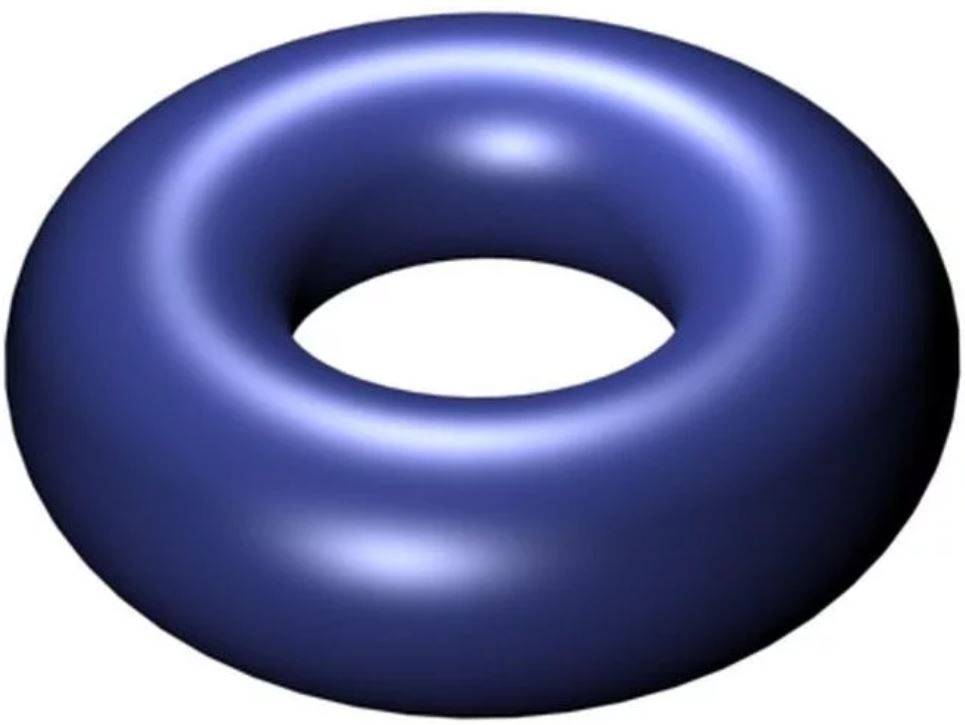
\includegraphics[width=\linewidth]{9I-2}
        \end{figure}
    \end{minipage}
\end{minipage}}
{НаписанноеРешение}
{ВерныйОтвет}{Подсказка}
\end{problem}

\begin{problem}{Масштаб.}{6.5.3}{6K}{(лёгкая)}
{Масштаб, указанный на карте, говорит, что $1$ см соответствует $900$ м.\\ Сколько сантиметров будет составлять расстояние между пунктами $A$ и $B$ на карте, если на местности расстояние между ними (по прямой) равно $4{,}05$ км?}
{НаписанноеРешение}
{ВерныйОтвет}{Подсказка}
\end{problem}

\begin{problem}{Масштаб.}{6.5.3}{6K}{(лёгкая)}
{Масштаб карты утверждает, что $1$ см соответствует $750$ м.\\ Сколько сантиметров будет составлять расстояние между городами $\Phi$ и $\Lambda$ на карте, если на местности между ними $3{,}84$ км?}
{НаписанноеРешение}
{ВерныйОтвет}{Подсказка}
\end{problem}

\begin{problem}{Масштаб.}{6.5.3}{6K \textcolor{red}{\textbf{$\spadesuit$}}}{(лёгкая)}
{Масштаб карты утверждает, что $1$ см соответствует $700$ м.\\ Сколько миллиметров будет составлять на карте расстояние между городами $\Pi$ и $\Lambda$, если их соединяет прямая дорога длиной $4{,}48$ км?}
{Поскольку один сантиметр на карте соответствует 700 метрам, выясним, сколько раз 700 м умещается в $4{,}48$ км. $4{,}48$ км $= 4480$ м. $4480 : 700 = \frac{448}{70} = \frac{224}{35} = \frac{32}{5} = 6{,}4$ раза. Таким образом, на карте расстояние между городами $\Pi$ и $\Lambda$ составляет $6{,}4$ сантиметра, или 64 миллиметра.}
{Расстояние между городами $\Pi$ и $\Lambda$ на карте составит 64 миллиметра.}{Сколько раз расстояние в 700 м <<умещается>> в $4{,}48$ км?}
\end{problem}

\begin{problem}{Масштаб.}{6.5.3}{6K}{(лёгкая)}
{Группа туристов планирует за день пройти расстояние, которое на навигаторе составляло $14$ километров $160$ метров. Однако навигатор разрядился, и у туристов осталась только обычная карта с масштабом $1 : 120000$ (в одном сантиметре на карте~--- $120000$ сантиметров).\\ Сколько миллиметров занимает на карте их маршрут?}
{В одном сантиметре на карте 120000 сантиметров, что то же самое, что и 1200 метров, или $1{,}2$ км. Общее расстояние составляет 14160 метров. Выясним, сколько раз в этом расстоянии умещается 1200 метров: $14160 : 1200 = 1416 : 120 = 708 : 60 = 354 : 30 = 177 : 15 = 59 : 5 = 11{,}8$ раз. Значит, на карте их маршрут занимает $11{,}8$ сантиметров, или, что то же самое, $118$ миллиметров.}
{Маршрут туристов на карте занимает 118 миллиметров.}{Сколько метров умещается в один сантиметр на карте?\\
Сколько всего таких расстояний надо пройти группе туристов?}
\end{problem}

\begin{problem}{Масштаб.}{6.5.3}{7A}{(лёгкая)}
{Масштаб карты таков, что в 1 см 700 м. Известно, что на карте расстояние между деревнями Э и Д по прямой составляет $7{,}1$ см.\\ Может ли дорога из Э в Д быть короче 5 км? 4 км? Насколько?}
{Если на карте расстояние между деревнями Э и Д по прямой составляет $7{,}1$ см, то в реальной жизни расстояние составит $7{,}1 \cdot 700 = 4970$ метров.\\
Это значит, что дорога из Э в Д может быть длиной 4970 метров (если она идёт по прямой), но никак не короче. Поэтому дорога может быть короче, чем 5 км (на 30 метров), а короче чем 4 километра она быть не может.}
{Дорога из деревни Э в деревню Д имеет длину как минимум 4970 метров. Отдельно отмечу, что если дорога виляет зигзагами (например, если она проходит через горы), то её длина может быть гораздо больше --- и 6, и 8, и 13 километров.}{Сколько метров по прямой от деревни Э до деревни Д?\\ Обязательно ли упомянутая в задаче дорога идёт по прямой?}
\end{problem}

\begin{problem}{Площадь треугольника.}{6.5.4}{6K}{(лёгкая)}
{У Жени был прямоугольник, ширина которого равна $4$, а периметр равен $48{,}5$. Вася решил, что это шоколадка, и разломал прямоугольник на множество маленьких кусочков. Известно, что Женя сумел собрать из всех этих кусочков квадрат (без дырок). Какова сторона у этого квадрата?}
{Сперва отметим, что поскольку периметр Жениного прямоугольника $P = 2(a + b)$, то сумма длины и ширины прямоугольника вдвое меньше периметра и составляет $48{,}5 : 2 = 24{,}25$ см.\\ Поэтому длина этого прямоугольника составляет $24{,}25 - 4 = 20{,}25$ см.\smallskip\\
Что мы знаем после действий Васи? Мы не знаем ни размеры частей, ни их форму, но мы знаем, что все части вместе составили квадрат. Какое хорошее свойство мы знаем про все части, взятые вместе? Мы знаем их площадь! Действительно, общая площадь не может ни уменьшиться, ни увеличиться (если только Вася не унёс с собой кусочек, но как нам известно, Женя собирал квадрат из всех кусков).\smallskip\\
Площадь у исходного прямоугольника равна $4 \cdot 20{,}25 = 80 + 1 = 81$ см$^2$.\\ Поэтому и у полученного квадрата площадь равна $81$ см$^2$. Следовательно, как мы знаем из таблицы умножения, сторона такого квадрата --- 9 сантиметров.}
{Сторона полученного квадрата равна 9 сантиметров.}{Какова длина и площадь исходного прямоугольника?\\ Какой факт мы можем использовать и почему?}
\end{problem}

\begin{problem}{Площадь треугольника.}{6.5.4}{6K \textcolor{red}{\textbf{$\spadesuit$}}}{(лёгкая)}
{Ширина прямоугольника~--- $8$ см, а длина~--- в $2{,}5$ раза больше ширины. Какова площадь у квадрата, имеющего такой же периметр, что и этот прямоугольник?}
{Раз длина в $2{,}5$ раза больше ширины, она равна $8 \cdot 2{,}5 = 20$ см. Мы знаем, что какой-то квадрат имеет такой же периметр, как и этот прямоугольник. А каков периметр у этого прямоугольника? Как и всегда, можем вычислить по известной формуле: $P = 2(a + b) = 2 \cdot (8 + 20) = 2 \cdot 28 = 56$ см. Если квадрат имеет периметр 56, то его сторона в 4 раза меньше и равна $56 : 4 = 14$ см.\\
Площадь у этого квадрата будет равна $14^2 = 14 \cdot 14 = 196$ см$^2$.}
{У такого квадрата площадь равна 196 см$^2$.}{Чему равны длина и периметр нашего прямоугольника?}
\end{problem}

\begin{problem}{Площадь треугольника.}{6.5.4}{6K}{(лёгкая)}
{\vspace{-14mm}\\\begin{minipage}{\linewidth}
    \begin{minipage}{0.71\linewidth}
    \vspace{8mm}
    Все четыре прямоугольника на рисунке справа обладают \\ замечательным свойством: длина каждого вдвое больше, чем его ширина.\smallskip\\ Периметр самого маленького прямоугольника равен $12$.\\ Чему равен периметр всей фигуры?

    \end{minipage}
    \hspace{0.02\linewidth}
    \begin{minipage}{0.24\linewidth}
        \begin{figure}[H]
        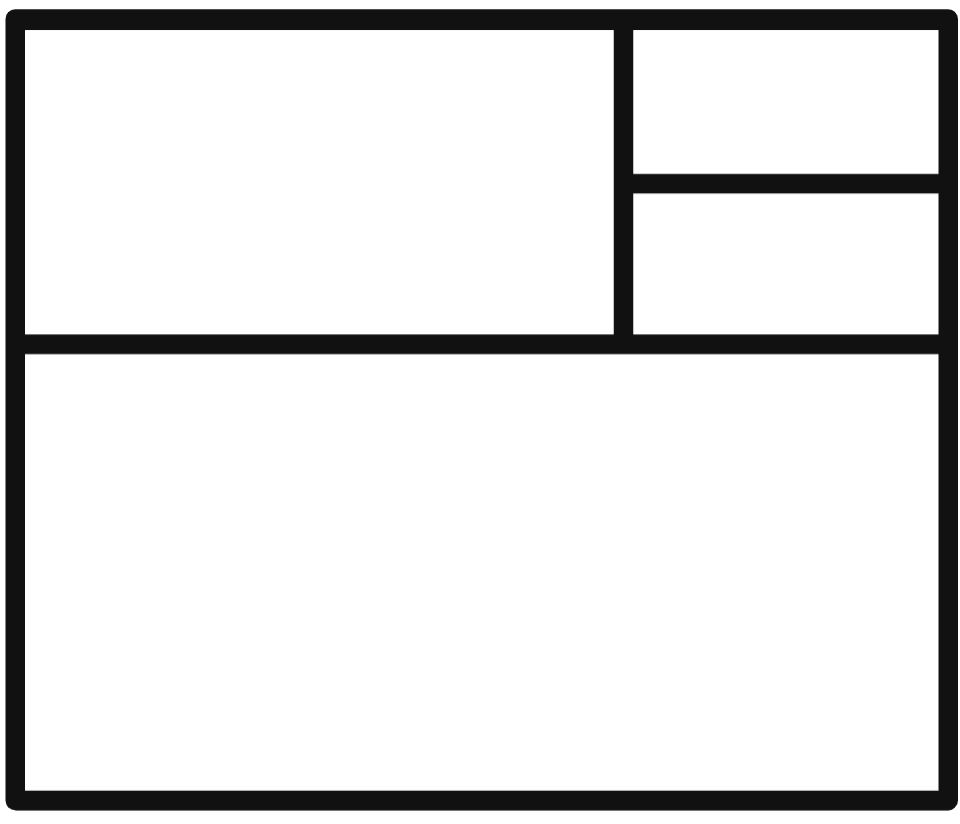
\includegraphics[width=\linewidth]{6K-29}
        \end{figure}
    \end{minipage}
\end{minipage}}
{Нам известно, что периметр самого маленького прямоугольника на рисунке равен 12. Значит, половина его периметра равна 6. Тогда, так как длина вдвое больше ширины, его длина должна быть равна 4, а ширина --- 2.\\ Смотрим на рисунок. Так как ширина равна 2, и два прямоугольника стоят вместе, ширина среднего прямоугольника равна $2 \cdot 2 = 4$. Тогда его длина вдвое больше и равна $4 \cdot 2 = 8$. Мы видим, что длина большого прямоугольника равна сумме длин среднего и маленького прямоугольников. Значит, она равна $4 + 8 = 12$.\\ Ширина вдвое меньше длины и поэтому равна $12 : 2 = 6$. Теперь мы знаем все размеры этой фигуры: её длина равна $12$, а ширина равна $6 + 2 + 2 = 10$. Следовательно, периметр фигуры равен $2(12 + 10) = 44$.}
{Периметр фигуры равен 44.}{Чему равна ширина самого маленького прямоугольника?}
\end{problem}

\begin{problem}{Площадь треугольника.}{6.5.4}{6K}{(лёгкая)}
{\vspace{-9mm}\\\begin{minipage}{\linewidth}
    \begin{minipage}{0.6\linewidth}
    \vspace{6mm}
    На рисунке справа, все четыре прямоугольника обладают замечательным свойством: длина каждого втрое больше, чем ширина.\smallskip\\ Периметр среднего прямоугольника равен 32 см. \\
    Чему равна площадь всей фигуры?

    \end{minipage}
    \hspace{0.04\linewidth}
    \begin{minipage}{0.35\linewidth}
        \begin{figure}[H]
        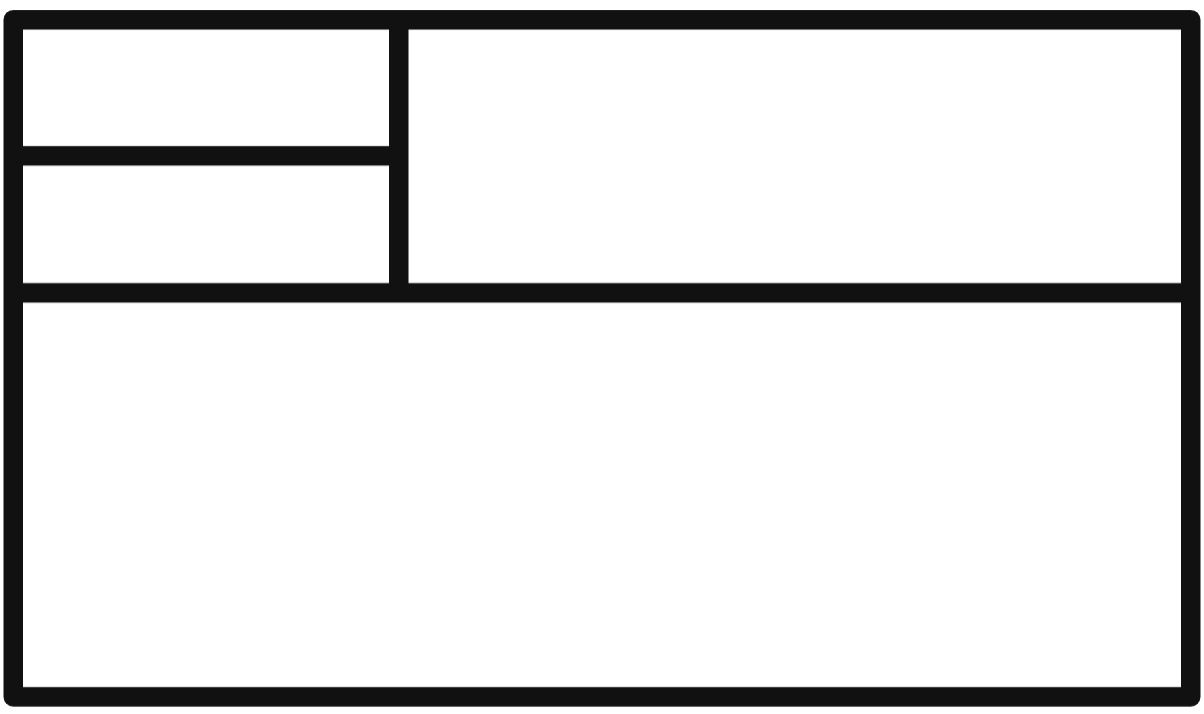
\includegraphics[width=\linewidth]{6K-30}
        \end{figure}
    \end{minipage}
\end{minipage}}
{Средний прямоугольник мы можем наблюдать в правом верхнем углу. Если его периметр равен 32 см, это значит, что сумма его длины и ширины равна 16 сантиметрам. А так как длина прямоугольника втрое больше ширины, это значит, что его ширина составляет 4 сантиметра, а длина~--- 12 сантиметров.\\ Тогда ширина у каждого из прямоугольников слева равна двум сантиметрам.\\ Следовательно, длина равна $2 \cdot 3 = 6$ сантиметров. Зная это, мы можем найти длину большого прямоугольника: она равна сумме длин маленького и среднего прямоугольников, то есть $6 + 12 = 18$ сантиметров. Поскольку и для него длина в три раза больше ширины, его ширина равна $18 : 3 = 6$ сантиметров.\\ Зная это, находим ширину всей фигуры: она равна $4 + 6 = 10$ сантиметров.\\
Таким образом, фигура~--- прямоугольник со сторонами 10 и 18 сантиметров.\\ Поэтому, её площадь равна 180 см$^2$.}
{Площадь данного прямоугольника равна 180 см$^2$.}{Чему равны стороны среднего прямоугольника?}
\end{problem}

\begin{problem}{Площадь треугольника.}{6.5.4}{6K \textcolor{red}{\textbf{$\spadesuit$}}}{(лёгкая)}
{У прямоугольника $ABCD$ ширина равна $8$ см, а длина больше ширины на $125\%$. Чему равен периметр квадрата, имеющего такую же площадь, как и этот прямоугольник?}
{НаписанноеРешение}
{ВерныйОтвет}{Подсказка}
\end{problem}

\begin{problem}{Площадь треугольника.}{6.5.4}{6K}{(лёгкая)}
{\vspace{-7mm}\\\begin{minipage}{\linewidth}
    \begin{minipage}{0.7\linewidth}
    \vspace{3mm}
    Квадрат с периметром $P = 240$ сантиметров разрезали на $24$ маленьких одинаковых прямоугольничка (см. рис.)\smallskip\\ Определить периметр и площадь маленьких прямоугольников.

    \end{minipage}
    \hspace{0.04\linewidth}
    \begin{minipage}{0.24\linewidth}
        \begin{figure}[H]
        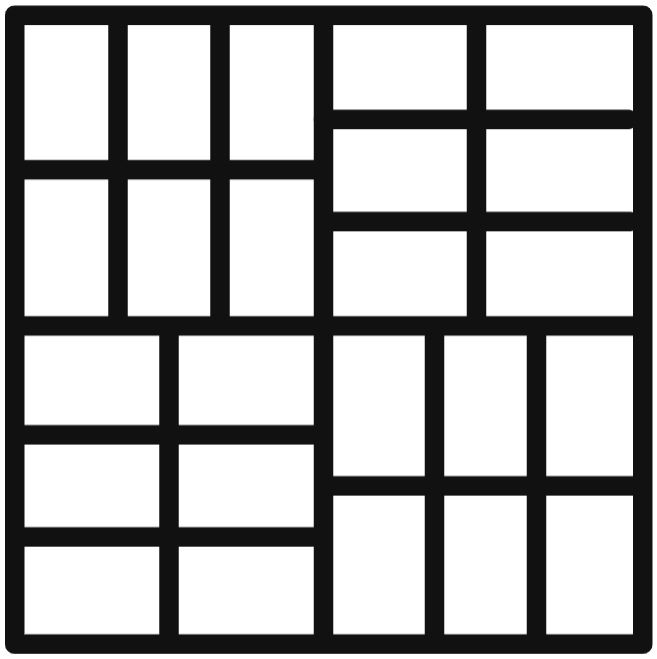
\includegraphics[width=\linewidth]{6K-10}
        \end{figure}
    \end{minipage}
\end{minipage}}
{НаписанноеРешение}
{ВерныйОтвет}{Подсказка}
\end{problem}

\begin{problem}{Площадь треугольника.}{6.5.4}{6K}{*}
{\vspace{-9mm}\\\begin{minipage}{\linewidth}
    \begin{minipage}{0.67\linewidth}
    \vspace{5mm}
    На рисунке справа изображен квадрат, который разделили на два неравных прямоугольника. \smallskip\\ Достоверно известно, что сумма периметров этих двух прямоугольников равна $54$ метрам.\\ Чему равна площадь этого квадрата?

    \end{minipage}
    \hspace{0.05\linewidth}
    \begin{minipage}{0.26\linewidth}
        \begin{figure}[H]
        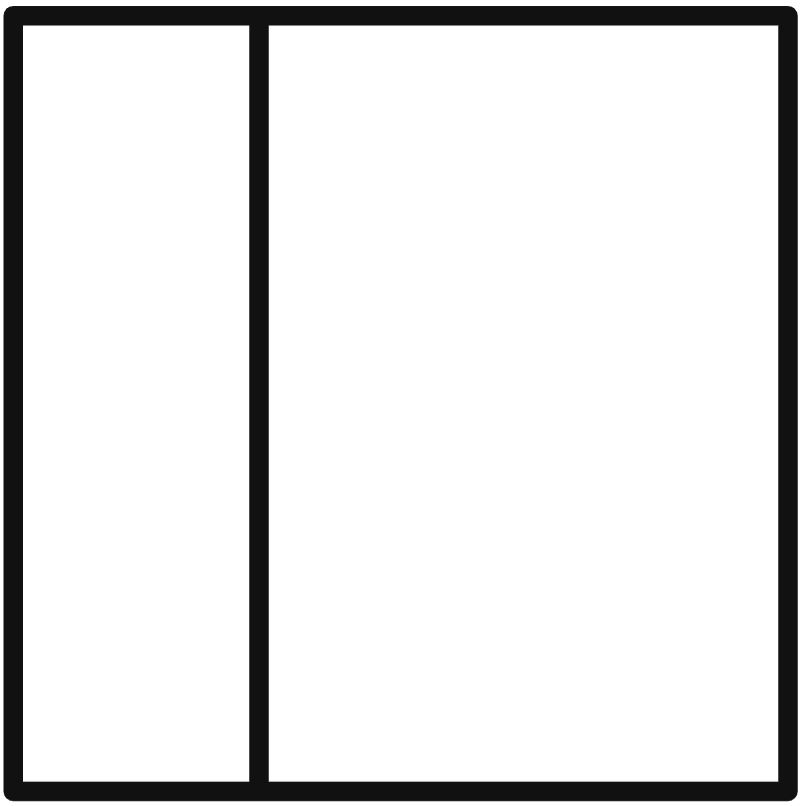
\includegraphics[width=\linewidth]{6K-32}
        \end{figure}
    \end{minipage}
\end{minipage}}
{Пусть сторона этого квадрата --- некоторое $a$ (в метрах). Для того, чтобы оградить эти два прямоугольника забором, понадобится $4a$ метров на вертикальные перегородки (по две у каждого прямоугольника) и ещё $2a$ на верхнюю и нижнюю стороны квадрата. Таким образом, общий периметр этих двух прямоугольников равен $4a + 2a = 6a$, что в 6 раз больше стороны этого квадрата. Значит, сторона этого квадрата равна $54 : 6 = 9$ м. Тогда площадь равна $S = 9^2 = 81$ м$^2$.}
{Площадь этого квадрата составляет 81 м$^2$.}{Пусть сторона этого квадрата --- некоторое $a$. Сколько таких сторон понадобится для того, чтобы получить суммарный периметр двух изображённых прямоугольников?}
\end{problem}

\begin{problem}{Площадь треугольника.}{6.5.4}{6K}{*}
{\vspace{-8mm}\\\begin{minipage}{\linewidth}
    \begin{minipage}{0.81\linewidth}
    \vspace{7mm}
    Для прямоугольников на рисунке справа известно, что площади двух маленьких прямоугольников равны друг другу и вместе составляют $\frac{4}{7}$ от площади среднего прямоугольника под ними. Средний же прямоугольник, в свою очередь, имеет площадь вдвое меньше, чем большой прямоугольник. \smallskip\\ Чему равна площадь всей фигуры (всех четырёх прямоугольников вместе), если известно, что ширина маленького прямоугольника равна $ \frac{5}{3}$, а длина равна $6$?

    \end{minipage}
    \hspace{0.02\linewidth}
    \begin{minipage}{0.15\linewidth}
        \begin{figure}[H]
        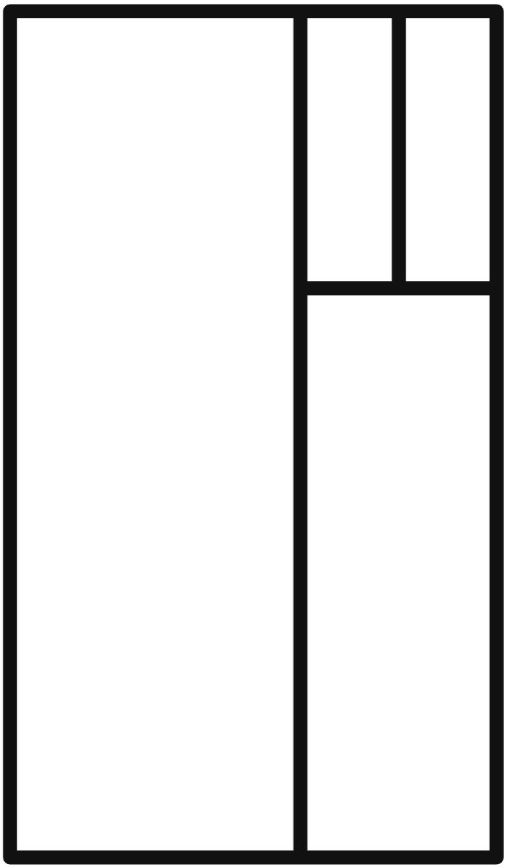
\includegraphics[width=\linewidth]{6K-31}
        \end{figure}
    \end{minipage}
\end{minipage}}
{Если у маленького прямоугольника ширина равна $\frac53$, а длина --- 6, площадь этого прямоугольника равна $\frac53\cdot6 = 10$.\\ Следовательно, площадь двух маленьких прямоугольников равна 20.\\ Значит, средний прямоугольник имеет площадь $20 \cdot\frac74 = 35$.\\ Большой прямоугольник имеет вдвое большую площадь $\Rightarrow$ его площадь равна 70.\\
Общая площадь всех четырёхугольников вместе равна $20 + 35 + 70 = 125$.}
{Площадь всей фигуры составляет 125.}{Чему равна площадь маленького прямоугольника?}
\end{problem}

\begin{problem}{Площадь треугольника.}{6.5.4}{6K}{(лёгкая)}
{Квадрат с периметром $48$ разрезали на шесть квадратов (не обязательно одинаковых). Каков общий периметр получившихся квадратов?}
{НаписанноеРешение}
{ВерныйОтвет}{Подсказка}
\end{problem}

\begin{problem}{Площадь треугольника.}{6.5.4}{6K}{(лёгкая)}
{Стороны прямоугольника равны $8$ и $10$. Найти площадь четырёхугольника, вершины которого расположены в серединах сторон данного прямоугольника.}
{НаписанноеРешение}
{ВерныйОтвет}{Подсказка}
\end{problem}

\begin{problem}{Площадь треугольника.}{6.5.4}{6K \textcolor{red}{\textbf{$\spadesuit$}}}{(лёгкая)}
{Из прямоугольника, одна сторона которого равна $21$ см, вырезали три квадрата с периметром $28$ см каждый. Площадь оставшейся фигуры в $9$ раз больше, чем сумма площадей всех вырезанных частей. Найти $S$ и $P$ прямоугольника.}
{НаписанноеРешение}
{ВерныйОтвет}{Подсказка}
\end{problem}

\begin{problem}{Площадь треугольника.}{6.5.4}{6K \textcolor{red}{\textbf{$\spadesuit$}}}{(лёгкая)}
{Длина прямоугольника равна 56 см, ширина прямоугольника составляет $\frac{4}{7}$ его длины. Чему (в см$^2$) равна площадь квадрата, имеющего такой же периметр, как и данный прямоугольник?}
{НаписанноеРешение}
{ВерныйОтвет}{Подсказка}
\end{problem}

\begin{problem}{Площадь треугольника.}{6.5.4}{6K \textcolor{red}{\textbf{$\spadesuit$}}}{(лёгкая)}
{Квадрат с периметром $56$ см разрезали на два прямоугольника. Периметр первого прямоугольника~--- $40$ см. Найдите периметр второго прямоугольника.}
{НаписанноеРешение}
{ВерныйОтвет}{Подсказка}
\end{problem}

\begin{problem}{Площадь треугольника.}{6.5.4}{6K \textcolor{red}{\textbf{$\spadesuit$}} кандидат на выпиливание вместе с остальной геомой на пифагора}{*}
{Удочка в длину занимает $5$ метров. Может ли человек с подобной
удочкой влезть в маршрутку? (для упрощения задачи считать, что маршрутка~--- пустая комната с прямыми углами размерами $3 \times 3 \times 4$ метра), прямоугольный параллелепипед. Сложить удочку нельзя, сломать можно, но жалко.}
{НаписанноеРешение}
{ВерныйОтвет}{Подсказка}
\end{problem}

\begin{problem}{Площадь треугольника.}{6.5.4}{6K}{*}
{\vspace{-8mm}\\\begin{minipage}{\linewidth}
    \begin{minipage}{0.5\linewidth}
    \vspace{2mm}
    Вычислить площадь фигур, которые изображены на клетчатой сетке справа.\smallskip\\ Считать, что 1 клетка $=$ 1 см.

    \end{minipage}
    \hspace{0.05\linewidth}
    \begin{minipage}{0.44\linewidth}
        \begin{figure}[H]
        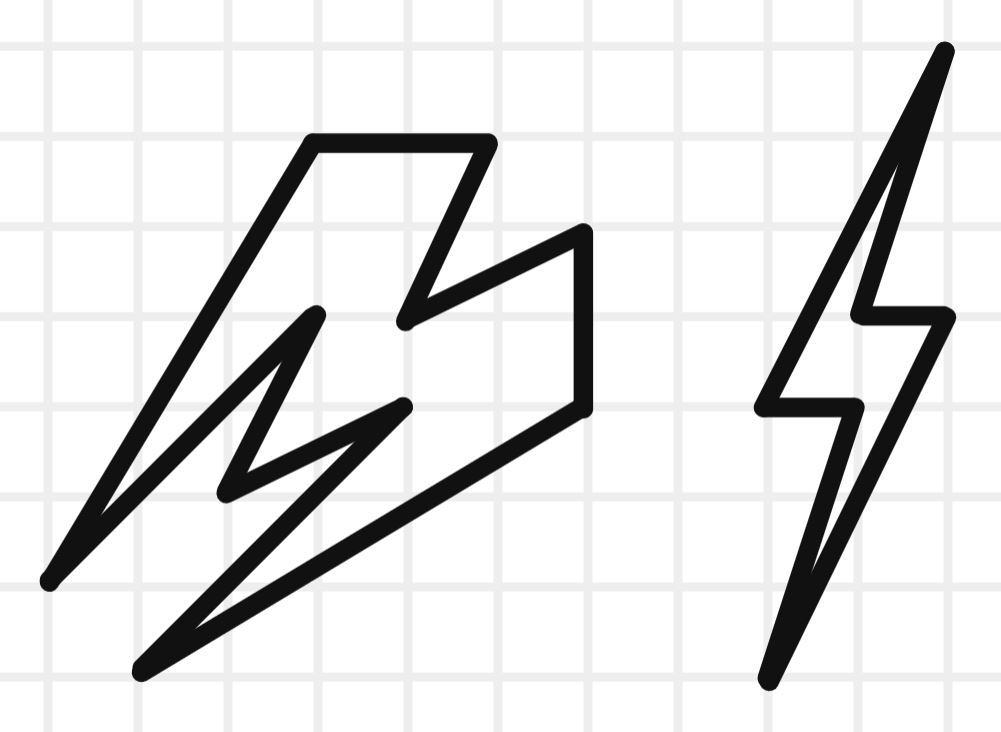
\includegraphics[width=\linewidth]{6K-35}
        \end{figure}
    \end{minipage}
\end{minipage}}
{НаписанноеРешение}
{ВерныйОтвет}{Подсказка}
\end{problem}

\begin{problem}{Площадь треугольника.}{6.5.4}{6K}{(лёгкая)}
{\vspace{-7mm}\\\begin{minipage}{\linewidth}
    \begin{minipage}{0.75\linewidth}
    \vspace{3mm}
    Из квадрата $5 \times 5$ см вырезали по центру квадрат так,\\ чтобы получилась рамка для фотографии (как на рисунке).\smallskip\\ Найди площадь рамки, если её толщина равна $1$ см.
    
    \end{minipage}
    \hspace{0.03\linewidth}
    \begin{minipage}{0.2\linewidth}
        \begin{figure}[H]
        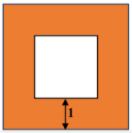
\includegraphics[width=\linewidth]{6K-22}
        \end{figure}
    \end{minipage}
\end{minipage}}
{НаписанноеРешение}
{ВерныйОтвет}{Подсказка}
\end{problem}

\begin{problem}{Площадь треугольника.}{6.5.4}{X}{*}
{\vspace{-5mm}\\\begin{minipage}{\linewidth}
    \begin{minipage}{0.54\linewidth}
    \vspace{2mm}
    Найди площадь фигуры, которая изображена на рисунке справа (2 клетки $=$ 1 см)

    \end{minipage}
    \hspace{0.05\linewidth}
    \begin{minipage}{0.4\linewidth}
        \begin{figure}[H]
        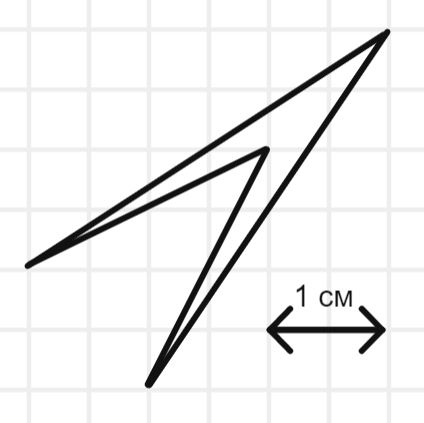
\includegraphics[width=\linewidth]{X-1}
        \end{figure}
    \end{minipage}
\end{minipage}}
{Несложно отметить, что вся фигура помещается в квадрат со стороной 3 сантиметра (на рисунке ниже отмечен фиолетовым).
\vspace{-5mm}\\\begin{minipage}{\linewidth}
    \begin{minipage}{0.54\linewidth}
    \vspace{6mm}
    Его площадь нам известна --- она составляет 9 см$^2$. Большие треугольники по краям (выделены синим) имеют площадь 3 (основание на высоту пополам). Маленькие треугольники (отмечены зелёным) имеют площадь 1, поскольку их основания равны 1 см, а высоты по 2 см.\\ Таким образом, общая площадь в 9 см$^2$ составляется из нашей фигуры, двух треугольников площадью 3 см$^2$ каждый, и двух треугольников площадью 1 см$^2$ каждый.

    \end{minipage}
    \hspace{0.05\linewidth}
    \begin{minipage}{0.4\linewidth}
        \begin{figure}[H]
        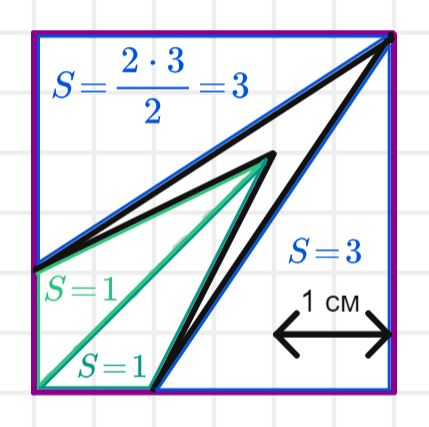
\includegraphics[width=\linewidth]{sol79}
        \end{figure}
    \end{minipage}
\end{minipage}
 Следовательно, площадь данной фигуры равна $9 - 3\cdot2 - 1\cdot2 = 9 - 8 = 1$ см$^2$.}
{Площадь данной фигуры равна 1 см$^2$.}{Посмотри на то, сколько данной фигуре не хватает до квадрата со стороной 3 сантиметра. Используй формулу для площади треугольника.}
\end{problem}

\begin{problem}{Приближенные значения. Округления.}{6.5.5}{6K letovo}{(лёгкая)}
{\vspace{-7mm}\\\begin{minipage}{\linewidth}
    \begin{minipage}{0.7\linewidth}

    На рисунке изображен круг, площадь которого равна $33$. \\ Чему может быть равна площадь фиолетовой части?
    \medskip\\ (A) 3; \hfill (B) 8; \hfill (C) 15; \hfill (D) 25; \hfill (E) $16\frac{1}{2}$.

    \end{minipage}
    \hspace{0.05\linewidth}
    \begin{minipage}{0.23\linewidth}
        \begin{figure}[H]
        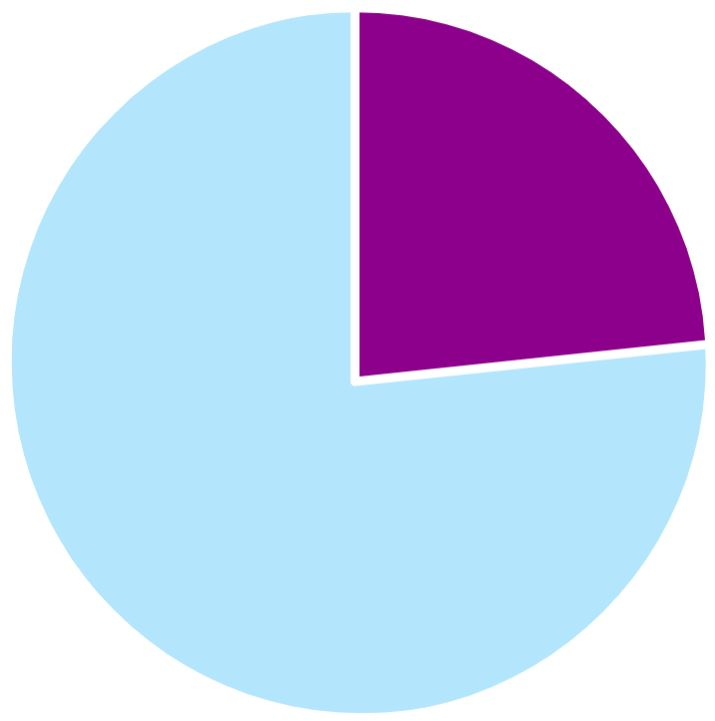
\includegraphics[width=\linewidth]{6K-21}
        \end{figure}
    \end{minipage}
\end{minipage}}
{Как видно из рисунка, фиолетовая часть составляет чуть меньше четверти от всего круга. Поскольку площадь всего круга равна 33, площадь четверти круга в 4 раза меньше и равна $33 : 4 = 8{,}25$. Поэтому, площадь фиолетовой части должна быть близка к этому числу, но чуть меньше $\Rightarrow$ правильный ответ --- (B)}
{Площадь фиолетовой части может быть равна 8 (ответ В).}{Чему равна площадь половины круга? Четверти?}
\end{problem}

\begin{problem}{Приближенные значения. Округления.}{6.5.5}{6S}{(лёгкая)}
{Из соснового дерева сделан кубик весом 8 г. Ребро кубика равно $2{,}5$ см.\\ Какой объём занимает $4{,}8$ т соснового дерева? Ответ округлить до $0{,}1$ м$^{3}$.}
{НаписанноеРешение}
{ВерныйОтвет}{Подсказка}
\end{problem}

\begin{problem}{Приближенные значения. Округления.}{6.5.5}{6S}{(лёгкая)}
{В одном математическом кружке девочек больше 91\% от общего числа участников. Найти наименьшее возможное количество участников кружка.}
{НаписанноеРешение}
{ВерныйОтвет}{Подсказка}
\end{problem}

\begin{problem}{Приближенные значения. Округления.}{6.5.5}{6K}{*}
{Для банка заказали сейф, имеющий форму прямоугольного параллелепипеда. Его высота~--- $1{,}5$ м, ширина~--- $1{,}6$ м, длина~--- $1{,}9$ м.\\ Какое наибольшое количество слитков золота, имеющих форму куба с ребром $6$ см, можно положить в этот сейф?}
{НаписанноеРешение}
{ВерныйОтвет}{Подсказка}
\end{problem}

\begin{problem}{Длина окружности, площадь круга.}{6.5.6}{6K}{(лёгкая)}
{\vspace{-7mm}\\\begin{minipage}{\linewidth}
    \begin{minipage}{0.7\linewidth}
    \vspace{8mm}
    На рисунке справа изображена схема водных каналов: равносторонний треугольник (то есть такой, что все его стороны равны) со стороной 4 км и три полуокружности.\\ Можно ли проплыть по всем шести каналам ровно по одному разу и вернуться в точку старта? \smallskip\\ Сколько километров (примерно) надо будет проплыть?

    \end{minipage}
    \hspace{0.05\linewidth}
    \begin{minipage}{0.23\linewidth}
        \begin{figure}[H]
        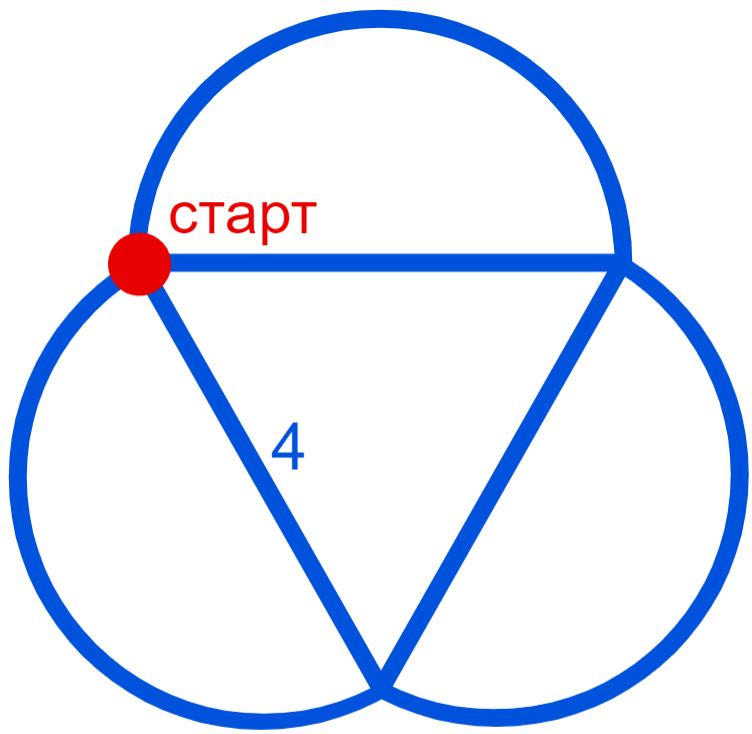
\includegraphics[width=\linewidth]{6K-11}
        \end{figure}
    \end{minipage}
\end{minipage}}
{Довольно быстро становится понятно, что составить такой маршрут можно: например, можно вначале проплыть по всему внутреннему треугольнику, а потом по трём наружним дугам. Для того, чтобы найти длину всего маршрута, найдём длины каналов: прямые каналы имеют длину 4 км. Дуги же являются частями окружностей с радиусом 2 км. И поскольку длина окружности равна $2\pi r$, половина длины окружности равна $\pi r$, а в нашем случае $\pi \cdot 2 = 2\pi$. Следовательно, длина всего маршрута составляет $L = 3\cdot4 + 3\cdot 2\pi = 12 + 6\pi$ км. Для того, чтобы вычислить приближённое значение, возьмём примерное значение $\pi \approx 3{,}14$. Получаем $L = 12 + 6 \cdot 3{,}14 = 12 + 18{,}84 = 30{,}84 \approx 31$ км.}
{Всего надо будет проплыть приблизительно 31 километр.\\
Отмечу, что если бы взяли более <<грубое>> приближение $\pi \sim 3$, мы бы получили ответ $12 + 6 \cdot 3 = 30$ км, потеряв целый километр. Поэтому обычно всегда используют приближение $\pi \approx 3{,}14$ --- в итоге ошибка не превышает $0{,}1\%$.}{Чему равны радиусы в этом случае? Используй известную формулу для длины окружности, чтобы получить формулу для длины полуокружности.}
\end{problem}

\begin{problem}{Длина окружности, площадь круга.}{6.5.6}{6K}{(лёгкая)}
{Радиус Земли составляет примерно 6400км. (Землю можно считать шариком)\\
1. Нарисовать Землю и её Южный и Северный полюса.\\
2. Определить расстояние между полюсами (здесь и далее считать, что $\pi \approx 3{,}14$)}
{НаписанноеРешение}
{ВерныйОтвет}{Подсказка}
\end{problem}

\begin{problem}{Длина окружности, площадь круга.}{6.5.6}{6K}{(лёгкая)}
{\vspace{-7mm}\\\begin{minipage}{\linewidth}
    \begin{minipage}{0.54\linewidth}
    \vspace{8mm}
    На рисунке справа изображён пятиугольник $OABCD$ и четверть окружности.\smallskip\\
    Масштаб рисунка таков, что одна клетка равна 1 сантиметру.\medskip\\
    1. Найти площадь пятиугольника $OABCD$.\\
    2. Найти площадь четверти окружности.\\
    3. Сравнить две полученные площади, сделать выводы.

    \end{minipage}
    \hspace{0.05\linewidth}
    \begin{minipage}{0.4\linewidth}
        \begin{figure}[H]
        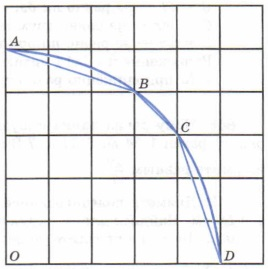
\includegraphics[width=\linewidth]{sol58}
        \end{figure}
    \end{minipage}
\end{minipage}}
{НаписанноеРешение}
{ВерныйОтвет}{Подсказка}
\end{problem}

\begin{problem}{Длина окружности, площадь круга.}{6.5.6}{6K}{(лёгкая)}
{Как известно, пиццы бывают разные~--- маленькие (диаметр 25 см), средние (диаметр 30 см), и большие (диаметр 35 см).\\ Что больше по площади: две маленьких пиццы или одна большая?}
{Найдём площади и того, и другого. Одна большая пицца имеет диаметр 35 сантиметров, то есть её радиус составляет $17{,}5$ сантиметров.\\ По формуле площади круга, площадь большой пиццы равна $\pi\cdot 17{,}5^2 = 306{,}25\pi$ квадратных сантиметров. (что примерно равно $306{,}25 \cdot 3{,}14 = 961{,}625 \approx 962$ см$^2$).\\ Радиус же маленькой пиццы равен $25 : 2 = 12{,}5$ сантиметров.\\ Площадь двух маленьких пицц равна $2\cdot \pi\cdot 12{,}5^2 = \pi \cdot 25 \cdot 12{,}5 = 312{,}5\pi$ см$^2$.\\ Это приблизительно равно $312{,}5 \cdot 3{,}14 = 981{,}25 \approx 981$ квадратный сантиметр.\\
Таким образом, $306{,}25\pi < 312{,}5\pi$, и площадь двух маленьких пицц больше одной большой пиццы. Хотя разница очень незначительна.}
{Площадь одной большой пиццы меньше площади двух маленьких пицц.\\
\textbf{Примечание:} Если посмотреть только на начинку пиццы, то есть не включать в площадь бортики пиццы (будем считать, что бортик имеет ширину в 1 сантиметр), то площадь начинки большой пиццы равна $\pi\cdot 16{,}5^2 = 272{,}25\pi$ см$^2$, а площадь начинки двух маленьких пицц уже равна $2\pi\cdot 11{,}5^2 = 264{,}5\pi$ см$^2$, и большая пицца оказывается больше двух маленьких.}{Используй формулу $S_{\text{круга}} = \pi r^2$.}
\end{problem}

\begin{problem}{Длина окружности, площадь круга.}{6.5.6}{6K}{(лёгкая)}
{Недалёкое будущее. Высокотехнологичная компания доставляет пиццу за 10 минут с помощью беспилотных дронов. Вася в дронах, к сожалению, не разбирается, но очень любит пиццу, в связи с чем ему нужна помощь в решении следующей практической задачки: пицца бывает маленькая, средняя, и большая.\\ Вася хочет знать, кусок какой пиццы больше всех, а какой~--- меньше всех.\smallskip\\ Помоги ему это определить, если известно, что маленькая пицца имеет диаметр 25 сантиметров, и её режут на 6 одинаковых кусков, средняя пицца имеет диаметр 30 сантиметров, и её режут на 8 одинаковых кусков, а большая пицца имеет диаметр 35 сантиметров, и её всегда режут на 10 абсолютно одинаковых кусков.}
{Используем формулу $S = \pi r^2$. Кусок маленькой пиццы в 6 раз меньше целой маленькой пиццы и потому имеет площадь $\frac16\cdot\pi\cdot 12{,}5^2 = \frac{625}{24}\pi$ см$^2$.\\ Средняя пицца: её кусок в 8 раз меньше целой средней пиццы, поэтому площадь одного куска равна $\frac18 \cdot \pi \cdot 15^2 = \frac{225}{8} \pi$ см$^2$. Кусок же большой пиццы меньше целой пиццы в 10 раз, и поэтому его площадь~--- $\frac{1}{10}\cdot\pi\cdot 17{,}5^2 = \frac{245}{8}\pi$ см$^2$.\\
$\frac{245}{8}\pi > \frac{225}{8}\pi = \frac{675}{24}\pi > \frac{625}{24}\pi$. То есть самым большим является кусок большой пиццы, а самым маленьким~--- кусок маленькой пиццы.}
{Самые большие куски~--- в большой пицце, а самые маленькие~--- в самой маленькой. (несмотря на то, что в самой большой пицце кусочки гораздо более узкие, эти куски всё равно больше всех остальных по площади).}{Используй формулу $S_{\text{круга}} = \pi r^2$ для каждой пиццы.\\ Во сколько раз кусок пиццы меньше площади целой пиццы в каждом случае?}
\end{problem}

\end{document}